\documentclass[letterpaper]{article} % DO NOT CHANGE THIS
\usepackage{aaai2026}  % DO NOT CHANGE THIS
\usepackage{times}  % DO NOT CHANGE THIS
\usepackage{helvet}  % DO NOT CHANGE THIS
\usepackage{courier}  % DO NOT CHANGE THIS
\usepackage[hyphens]{url}  % DO NOT CHANGE THIS
\usepackage{graphicx} % DO NOT CHANGE THIS
\usepackage{subcaption}
\urlstyle{rm} % DO NOT CHANGE THIS
\def\UrlFont{\rm}  % DO NOT CHANGE THIS
\usepackage{natbib}  % DO NOT CHANGE THIS AND DO NOT ADD ANY OPTIONS TO IT
\usepackage{caption} % DO NOT CHANGE THIS AND DO NOT ADD ANY OPTIONS TO IT
\frenchspacing  % DO NOT CHANGE THIS
\setlength{\pdfpagewidth}{8.5in} % DO NOT CHANGE THIS
\setlength{\pdfpageheight}{11in} % DO NOT CHANGE THIS

%
% Keep the \pdfinfo as shown here. There's no need
% for you to add the /Title and /Author tags.
\pdfinfo{
/TemplateVersion (2026.1)
}

\setlength{\belowcaptionskip}{-5pt} % save space

\usepackage{amsmath, amssymb, amsthm}
\usepackage{stackengine}
\usepackage{longtable}
\usepackage{booktabs}
\usepackage{pdflscape}
\usepackage{multirow}
\usepackage{color}

\usepackage{algorithm}
\usepackage{algorithmicx}
\usepackage{algpseudocode}

\urlstyle{rm}
\def\UrlFont{\rm}


\newcommand{\mcomment}[2]{{\color{blue}\textbf{(#1)}}\footnote{\textbf{#1:} #2}}
\newcommand{\jules}[1]{\mcomment{Jules}{#1}}
\newcommand{\jeremie}[1]{\mcomment{Jérémie}{#1}}
\newcommand{\yann}[1]{\mcomment{Yann}{#1}}
% Metadata
% \pdfinfo{
% /TemplateVersion (2025.1)
% }

\setcounter{secnumdepth}{0} % Numbered sections



\title{Learning-Guided Simulated Annealing for the Capacitated Vehicle Routing Problem}

\author{
Jules Andretti,
Jérémie Cabessa,
Yann Strozecki
}

\affiliations{
David Laboratory, University of Versailles Saint-Quentin (UVSQ) – Université Paris-Saclay\\
78000 Versailles, France \smallskip\\
\{jules.andretti, jeremie.cabessa, yann.strozecki\}@uvsq.fr
}

\begin{document}

\maketitle

\begin{abstract}
The Capacitated Vehicle Routing Problem (CVRP) is a fundamental NP-hard combinatorial optimization problem with broad practical relevance. We propose \emph{Learning-Guided Simulated Annealing} (LG-SA), a hybrid framework that augments classical Simulated Annealing with a lightweight neural policy trained via Proximal Policy Optimization (PPO). The policy, a two-stage conditional MLP, learns to propose promising node-insertion moves from a rich, dynamic node-centric feature representation capturing local geometry, capacity status, and search meta-information. Feasibility is enforced by proactive action masking. On the standard $N=100$ Nazari benchmark, LG-SA achieves a routing cost of $16.343$ at $10{,}000$ steps and $15.81$ at $1{,}000{,}000$ steps, competitive with state-of-the-art neural improvement methods at a fraction of their inference time. On CVRPLIB Set~X, it reaches a $4.21\%$ average optimality gap without augmentation. The method scales near-linearly to instances of $N=10{,}000$ nodes and processes $10{,}000$ diverse instances in 31 minutes on a single GPU.
\end{abstract}


\section{Introduction}

The Capacitated Vehicle Routing Problem (CVRP) \citep{dantzig_truck_1959} is one of the most intensively studied problems in combinatorial optimization. It models the task of designing a set of minimum-cost vehicle routes to serve geographically distributed customers subject to vehicle capacity constraints, and arises naturally in logistics, supply chain management, and urban mobility planning. Despite decades of research, the NP-hard nature of CVRP means that scaling exact solvers to real-world instance sizes remains computationally intractable \citep{toth_vehicle_2002}.

Classical heuristics --- from the Clarke-Wright savings algorithm \citep{clarke_scheduling_1964} to iterative local search operators such as 2-opt --- provide practical solutions but often require extensive expert tuning and exhibit limited generalization across problem distributions \citep{liu_heuristics_2023}. Metaheuristics such as Simulated Annealing (SA) \citep{kirkpatrick_optimization_1983} improve over greedy descent by allowing controlled uphill moves via the Metropolis criterion, but their performance remains sensitive to temperature scheduling and the quality of the move proposal distribution.

The success of deep learning has inspired a new paradigm of \emph{neural combinatorial optimization} (NCO). \emph{Construction methods} build solutions autoregressively using attention-based encoders, achieving strong results on uniform instances \citep{nazari_reinforcement_2018, kool_attention_2019, kwon_pomo_2021}. \emph{Improvement methods}, by contrast, iteratively refine existing solutions through a learned local search, typically formulated as a Markov Decision Process (MDP) trained with reinforcement learning (RL). Prominent examples include the Dual-Aspect Collaborative Transformer (DACT) \citep{ma_learning_2021}, which employs a specialized heavyweight Transformer to learn the entire move-selection policy, and neighborhood-search approaches based on graph attention \citep{gao_learn_2020, wu_learning_2022}. While powerful, these models often carry a substantial computational footprint at inference time.

A complementary and more recent direction is \emph{Neural Simulated Annealing} (NSA) \citep{correia_neural_2023}, which retains the classical SA skeleton but replaces its uniform random move proposal with a learned distribution parameterized by a lightweight, permutation-equivariant network. By preserving the Metropolis-Hastings acceptance criterion, NSA retains SA's convergence properties while dramatically improving the informativeness of proposed moves. However, NSA has so far been validated only on unconstrained problems --- TSP, Knapsack, and Bin Packing --- and its extension to CVRP is non-trivial: vehicle capacity constraints render many candidate moves infeasible, and naïve rejection of infeasible proposals wastes both compute and learning signal.

\textbf{This paper bridges that gap.} We introduce \emph{Learning-Guided Simulated Annealing for CVRP} (LG-SA), which extends the NSA framework to the multi-route, capacity-constrained setting. Rather than deploying a heavyweight Transformer, we deliberately maintain a lightweight two-stage MLP policy that scores node pairs in $\mathcal{O}(N)$ time, enabling efficient GPU-batched parallel search over thousands of instances simultaneously. Our contributions are:

\begin{itemize}
    \item \textbf{Feasibility strategy analysis.} We systematically compare three constraint-handling strategies --- proactive action masking, reactive rejection, and indirect permutation with greedy reconstruction --- across three local search operators. We find that insertion with proactive masking consistently dominates, and characterize the underlying failure modes of the alternatives.

    \item \textbf{Dynamic node-centric feature representation.} We design a feature vector that enriches static node properties with dynamic signals: local geometry (detour cost and immediate neighbor coordinates), capacity status (route load ratio and slack), and SA meta-features (current temperature and search progress). An ablation study pinpoints which signals are critical, which are noisy, and which are redundant.

    \item \textbf{Shallow curriculum learning for lightweight policies.} We show that the optimal curriculum depth for a lightweight improvement policy ($\xi_{\text{CL}} \approx 120$ pre-steps) is far shallower than the $\xi_{\text{CL}}=2{,}500$ optimum reported for heavyweight constructive architectures. Deeper curricula induce catastrophic forgetting of the global cost landscape, a failure mode specific to small-capacity networks.

    \item \textbf{Comprehensive empirical evaluation.} Through extensive ablation studies covering features, reward formulations, network size, temperature scheduling, initialization strategy, and the Metropolis criterion itself, we rigorously quantify each design choice's contribution to final performance.
\end{itemize}

LG-SA achieves a routing cost of $16.343$ at $10{,}000$ steps and $15.81$ at $1{,}000{,}000$ steps on the standard Nazari $N=100$ benchmark, competitive with state-of-the-art neural improvement methods. On CVRPLIB Set~X, it reaches a $4.21\%$ average optimality gap without augmentation, and processes $10{,}000$ structurally diverse instances in 31 minutes on a single GPU. The method scales near-linearly from $N=10$ to $N=10{,}000$, confirming its practical tractability.

The paper is organized as follows. The \textit{Background and Related Work} section surveys related literature. The \textit{Problem Definition} section formally defines the CVRP. The \textit{Proposed Method} section describes the LG-SA framework: the neural architecture, feasibility strategies, and PPO training procedure. The \textit{Experimental Results} section presents our empirical evaluation. The \textit{Conclusion} section discusses limitations and future directions.

\section{Background and Related Work}

Since its introduction by \citet{dantzig_truck_1959}, the Capacitated Vehicle Routing Problem (CVRP) has been a central challenge in combinatorial optimization. While exact algorithms like branch-and-cut and branch-and-price are effective for small instances, the NP-hard nature of the problem makes them computationally intractable at scale \citep{toth_vehicle_2002}. This limitation has necessitated the use of heuristic approaches, ranging from constructive methods like Clarke-Wright \citep{clarke_scheduling_1964} to local search operators such as 2-opt. Metaheuristics like Simulated Annealing (SA) \citep{kirkpatrick_optimization_1983} and general solvers like OR-Tools \citep{ortools_routing} offer robust alternatives, yet often require extensive parameter tuning and domain expertise to ensure consistent performance across diverse instances \citep{liu_heuristics_2023, muriyatmoko_heuristics_2024}.

The success of deep learning in other domains has inspired two primary paradigms for neural combinatorial optimization: \textit{construction methods} and \textit{improvement methods}.

Construction methods build solutions from scratch. Pioneering work by \citet{nazari_reinforcement_2018} adapted pointer networks for VRPs by replacing recurrent encoders with attention mechanisms to handle dynamic state elements. \citet{kool_attention_2019} further advanced this with the Attention Model (AM), a Transformer-based architecture trained via REINFORCE, which showed strong performance across routing tasks like TSP and VRP without relying on RNNs.

Improvement methods, by contrast, refine existing solutions through iterative local search. These approaches generally formulate the improvement process as a Markov Decision Process (MDP). For instance, \citet{wu_learning_2022} developed a Transformer-based model where actions correspond to selecting node pairs for local operators like 2-opt. However, standard Transformer architectures often struggle to capture the inherent circularity of routing solutions. To address this, \citet{ma_learning_2021} introduced the Dual-Aspect Collaborative Transformer (DACT). DACT revisits solution representation by decoupling node and positional embeddings to minimize noise and distinctively employs a Cyclic Positional Encoding (CPE) based on Gray codes to explicitly model the circular symmetry of VRP tours. Trained via Proximal Policy Optimization (PPO) with a curriculum learning strategy, DACT effectively replaces the heuristic logic with a specialized, ``heavyweight'' neural policy that demonstrates superior generalization compared to previous Transformer-based models.

Other improvement approaches focus on learning specific heuristic components. \citet{gao_learn_2020} utilized a modified Graph Attention Network (EGATE) to learn Very Large Neighborhood Search (VLNS) heuristics, training destruction and repair operators with PPO to handle large-scale instances. Hybrid methods have also emerged: \citet{garcia-torres_combining_2022} proposed CDCP, combining a deep constructor with a deep perturbator to outperform purely constructive or improvement-based baselines. Similarly, \citet{bui_imitation_2023} introduced Imitation Improvement Learning (IIL), using classical heuristics (HGS, VNS) as expert demonstrators for imitation learning, scaling effectively to instances with up to 30,000 nodes.

Most closely related to our work is the Neural Simulated Annealing (NSA) framework proposed by \citet{correia_neural_2023}. Unlike DACT, which replaces the heuristic with a complex Transformer, NSA retains the classical Simulated Annealing metaheuristic but enhances it by learning a proposal distribution (policy). NSA frames SA as an MDP and uses lightweight, permutation-equivariant neural networks (often simple MLPs) to suggest moves, preserving the convergence guarantees of the Metropolis-Hastings acceptance criterion. While NSA has demonstrated strong performance on problems like Knapsack, Bin Packing, and TSP, it has primarily been tested with simple unconstrained operators and has not yet been adapted to the CVRP, where complex capacity constraints render many local moves infeasible. Our work seeks to bridge this gap, extending the lightweight, learnable proposal framework of NSA to the constrained domain of CVRP.

\section{Problem Definition}
\label{sec:problem_definition}

The \textit{Capacitated Vehicle Routing Problem (CVRP)} is defined on a complete undirected graph $G = (V, E)$, where $V = \{0\} \cup \mathcal{C}$ and $E = V \times V$ denote the sets of nodes and edges, respectively. Node $0$ corresponds to the central depot, and $\mathcal{C} = \{1, \dots, N\}$ represents the set of $N$ customers.

Each edge $(i, j) \in E$ is associated with a travel cost $c_{ij} = \|\mathbf{p}_i - \mathbf{p}_j\|_2$ (the Euclidean distance between 2D coordinates $\mathbf{p}_i, \mathbf{p}_j \in [0,1]^2$), satisfying $c_{ij} = c_{ji}$. Each customer $i \in \mathcal{C}$ has a non-negative demand $q_i$, while the depot has zero demand ($q_0 = 0$). An unlimited fleet of identical vehicles, each with uniform capacity $Q$, is stationed at the depot; the number of routes $m$ is therefore a decision variable unconstrained from above.

A route $R_k = (0, v_1, v_2, \ldots, v_p, 0)$ is a simple cycle (tour) starting and ending at the depot, where $\{v_1, \ldots, v_p\} \subseteq \mathcal{C}$ denotes the subset of customers served by vehicle $k$. A \textit{solution} $s = \{R_1, \ldots, R_m\}$ consists of a set of $m$ routes. A solution $s$ is considered \textit{feasible} if and only if it satisfies the following conditions:
\begin{enumerate}
    \item Each customer is visited exactly once by a single vehicle,
    $$
    \sum_{k=1}^{m} \mathbf{1}_{\{i \in R_k\}} = 1, \quad \forall i \in \mathcal{C} .
    $$
    \item For every route $R_k$, the total demand of its customers does not exceed the vehicle capacity $Q$, i.e.,
    $$
    \sum_{i \in R_k \setminus \{0\}} q_i \leq Q, \quad \forall k = 1, \ldots, m.
    $$
\end{enumerate}
The set of \textit{feasible solutions} is denoted by $\mathcal{F}$.

Let $x_{ij}(s)$ be a binary indicator variable defined by $x_{ij}(s) = 1$ if edge $(i,j)$ is traversed in any route $R_k$ of $s$, and $x_{ij}(s) = 0$ otherwise. The objective of the CVRP is to find a feasible solution $s^* \in \mathcal{F}$ that minimizes the total travel cost $C(s)$:
$$
s^* = \arg\min_{s \in \mathcal{F}} \Big\{ C(s) = \sum_{i \in V} \sum_{j \in V, i < j} c_{ij} x_{ij}(s) \Big\}
$$

\section{Proposed Method}

\subsection{Overview}

We propose a hybrid metaheuristic that combines a \textit{Simulated Annealing (SA)} process with a lightweight \textit{Neural Reinforcement Learning (RL) policy}. Adopting the Neural Simulated Annealing framework \citep{correia_neural_2023}, our method utilizes the SA component to orchestrate the global exploration of the solution space, ensuring convergence guarantees. Meanwhile, a trained neural network (NN) adaptively guides the selection of neighboring solutions, serving as a learnable proposal distribution. This approach contrasts with ``heavyweight'' architectures like the Dual-Aspect Collaborative Transformer (DACT) \citep{ma_learning_2021}, which employ deep encoders to replace the heuristic logic entirely, whereas our policy remains lightweight to minimize computational overhead.

\textit{Simulated Annealing} (SA) is a stochastic optimization heuristic that iteratively explores the neighborhood of a current solution. Given a solution $s$, SA samples a neighboring solution $s' \in \mathcal{N}(s)$ and accepts it according to the \textit{Metropolis criterion}: improving moves are always accepted, while worsening moves are accepted with probability $\exp(-\Delta C / T)$. Here, $\Delta C = C(s') - C(s)$ represents the cost difference, and $T$ is the temperature parameter. This stochastic acceptance, regulated by the annealing of $T$, allows the search to escape local optima.

In our framework, the sampling of a neighboring solution $s' \in \mathcal{N}(s)$ is no longer uniform but instead follows a probability distribution learned by the neural network. Formally, let $H: \mathcal{S} \times \mathcal{A} \to \mathcal{S}$ denote a \textit{neighborhood operator} that, for each solution $s \in \mathcal{S}$ and possible action $a \in \mathcal{A}(s)$ on $s$, produces the neighboring solution $s' = H(s, a) \in \mathcal{S}$. For instance, $a \in V \times V$ may represent a pair of edges (e.g., a 2-opt move), and $s' = H(s, a)$ is the solution obtained by exchanging those edges in $s$. The neighborhood of $s$ is thus defined as:
$$
\mathcal{N}(s) = \left\{ H(s, a) : a \in \mathcal{A}(s) \right\}.
$$
In classical SA, the neighboring solution $s'$ is obtained through \textit{uniform sampling} over the available moves. By contrast, we parameterize the proposal distribution as a policy $\pi_\theta$. The network learns a probability distribution $\pi_\theta(\cdot \mid s) \in \Delta(\mathcal{A}(s))$ over the feasible actions, and the neighboring solution is selected according to:
\begin{align*}
a \sim \pi_\theta(\cdot \mid s) \quad \text{ and } \quad s' = H(s, a) \in \mathcal{N}(s).
\end{align*}
The neural policy is learned via \textit{Reinforcement Learning (RL)} using \textit{Proximal Policy Optimization (PPO)}. PPO has proven effective for training improvement heuristics by providing stable policy updates and efficient sample usage.

To control the temperature $T$ in SA, we employ a \textit{geometric} (or \textit{lambda}) schedule. This is defined as:
$$
T_{k+1} = \alpha \, T_k, \quad \text{with } \alpha = \left( T_\mathrm{final} / T_0 \right)^{1/S}.
$$
This setting ensures a consistent decay from an initial temperature $T_0$ to a final temperature $T_\mathrm{final}$ over the $S$-step search horizon. Empirically, monotonic schedules often perform best for this class of hybrid solvers, motivating our adoption of the geometric schedule. The overall procedure is summarized in Algorithm~\ref{alg:learning_guided_sa_conceptual}.

\begin{algorithm}[h!]
\begin{algorithmic}[1]
\caption{Overview of the Learning-Guided SA}
\label{alg:learning_guided_sa_conceptual}
\Require Initial solution $s$, learned neural policy $\pi_\theta$, neighborhood operator $H$
\State Initialize $s^*$ and SA parameters (e.g., $T$)

\While{SA termination criterion not met}
    \State \textit{1. Model-Guided Neighbor Generation}
    \State \quad Encode current solution $s$
    \State \quad Sample action from policy: $a \sim \pi_\theta(a \mid s)$
    \State \quad Generate candidate solution: $s' \gets H(s, a)$
    
    \State \textit{2. Standard SA Procedure}
    \State \quad $s \gets \text{SA\_accept}(s, s', T)$ 
    \State \quad Update $T$ and $s^*$
\EndWhile

\State \Return $s^*$
\end{algorithmic}
\end{algorithm}

\subsection{Neural Model}
\label{Neural Model}

\paragraph{Generalities.}

The \textit{neural model} guides the selection of neighboring solutions. Given a current solution $s$, it assigns a score $z_{ij}$ to each candidate pair of customers (nodes) $(i, j)$. This score reflects the estimated likelihood that modifying $s$ through the pair $(i, j)$ will yield an improved solution $s'$. An action $a = (i, j)$ is then sampled according to the probability distribution induced by the scores $z_{ij}$, and the neighboring solution is obtained as $s' = H(s, a)$. The neural model is illustrated in Figure~\ref{fig_LG-SA}.


\begin{figure*}[t]
\centering
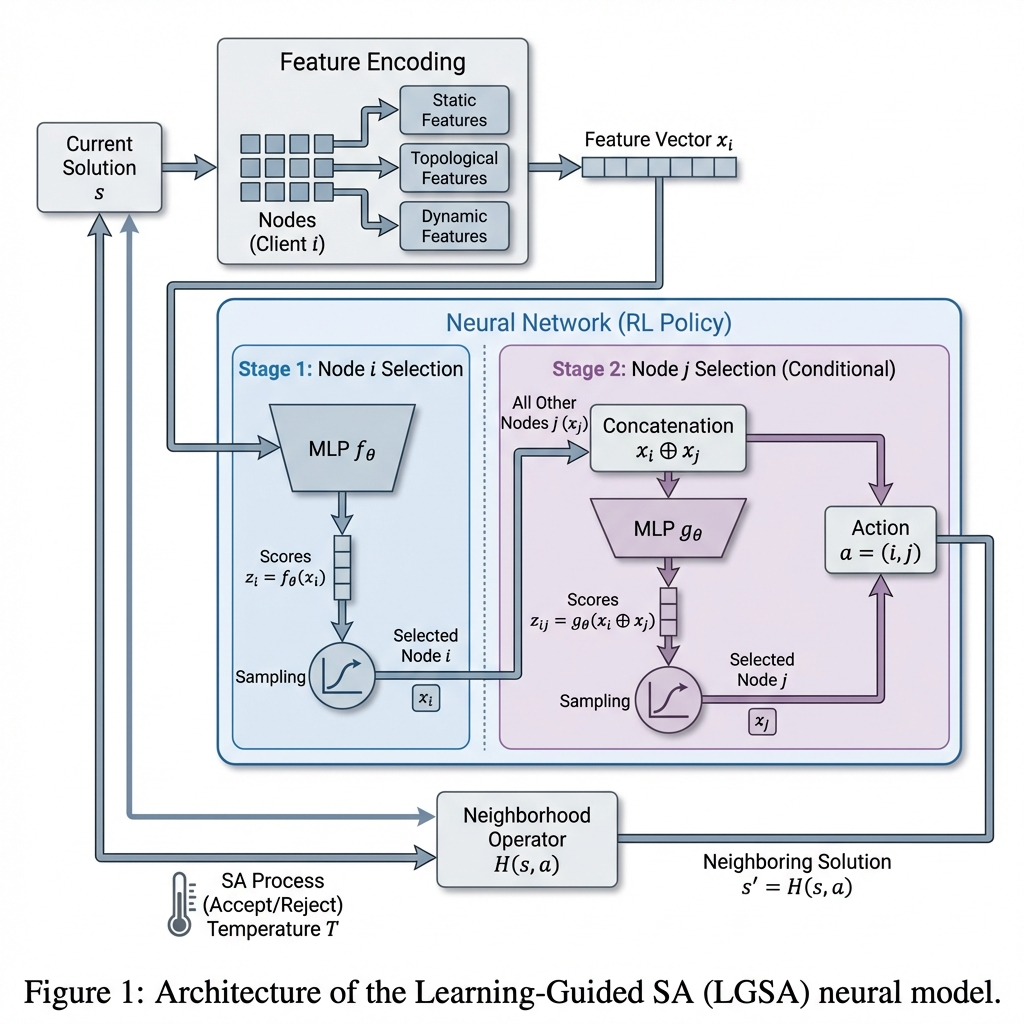
\includegraphics[width=0.8\textwidth]{pipline.png}
\caption{All $N$ nodes of the current solution $s$ are encoded and processed by the lightweight neural network in two sequential stages. In the first stage, every node is scored independently to select node $i$; in the second stage, node $i$'s embedding is concatenated with each remaining node to score and select node $j$. The resulting pair $a=(i,j)$ is sampled and yields the neighboring solution $s' = H(s,a)$.}
\label{fig_LG-SA}
\end{figure*}

\paragraph{Neighborhood operators.}

We consider three standard neighborhood operators defined over a pair of nodes $(i, j)$. In our framework, the operator is fixed: each experiment uses a single operator $H$ during both training and testing. The neural policy is therefore trained to learn a distribution tailored to that operator. The available operators are:

\begin{itemize}
    \item \textit{Swap:} Exchanges the positions of nodes $i$ and $j$, either within the same route or across different routes.
    \item \textit{Insertion (Relocation):} Removes node $i$ from its current position and reinserts it immediately after node $j$.
    \item \textit{2-opt / 2-opt*:} A unified operator that adapts based on route membership. For intra-route moves, it performs a standard 2-opt by removing edges $(i, \text{succ}(i))$ and $(j, \text{succ}(j))$ and reversing the enclosed path segment. For inter-route moves, it executes a 2-opt* (tail swap) by exchanging the trajectory suffixes following $i$ and $j$, creating new connections $(i, \text{succ}(j))$ and $(j, \text{succ}(i))$.
\end{itemize}

\paragraph{Input Representation.}
We consider two-dimensional (2D) CVRP instances with coordinates normalized to $[0, 1]$. To ensure \textit{scale invariance} and applicability to any problem size $N$, we utilize a \textit{node-centric} representation where each client $i$ is encoded via a local feature vector $\mathbf{x}_i$. Unlike standard approaches, our representation is enriched with dynamic ``quality'' signals that explicitly characterize the efficiency of the current solution state. Formally, $\mathbf{x}_i$ concatenates static, topological, capacity, and meta features as follows:

\begin{equation*}
\begin{split}
    \mathbf{x}_i = \Big[
        & \underbrace{\mathbf{p}_i, \theta_i, d_{i0}, \mathbf{1}_{\{i=0\}}, \tfrac{q_i}{Q}}_{\text{Static}}, \,
          \underbrace{\rho^{(5)}_i, \rho^{(10\%)}_i, \rho^{(33\%)}_i}_{\text{Spatial Density}}, \,
          \underbrace{\mathbf{p}_{i-1}, \mathbf{p}_{i+1}}_{\text{Topology}}, \\
        & \underbrace{\Delta^{\text{detour}}_i, d_{i, \text{cent}}}_{\text{Local Geometry}}, \,
          \underbrace{L_{r}, S_{r}, \eta_i}_{\text{Capacity Status}}, \,
          \underbrace{T, \tau}_{\text{Meta}}
    \Big].
\end{split}
\end{equation*}

Here, the \textit{Static} features include the node's coordinates $\mathbf{p}_i$, its polar coordinates relative to the depot $(\theta_i, d_{i0})$, a depot indicator flag $\mathbf{1}_{\{i=0\}}$, and the normalized demand $q_i/Q$. The remaining features describe the node's dynamic context within the current solution state:
\begin{itemize}
    \item \textit{Spatial Density:} The mean distance to the $k$-nearest neighbors, evaluated at $k=5$, $10\%$, and $33\%$ of the total node count $N$ (denoted $\rho^{(5)}_i, \rho^{(10\%)}_i, \rho^{(33\%)}_i$), capturing local neighborhood clustering.
    \item \textit{Topology:} The coordinates of the immediate predecessor $\mathbf{p}_{i-1}$ and successor $\mathbf{p}_{i+1}$ in the current route sequence.
    \item \textit{Local Geometry:} The \textit{detour cost} $\Delta^{\text{detour}}_i = d_{i-1, i} + d_{i, i+1} - d_{i-1, i+1}$ (measuring the geometric penalty of inserting node $i$) and the distance to the route's geometric centroid $d_{i, \text{cent}}$ (identifying spatial outliers).
    \item \textit{Capacity Status:} Let route $r$ be the route currently servicing node $i$, with total load $Q_r$. This block includes the Route Load Ratio $L_r = Q_r/Q$, the Capacity Slack $S_r = (Q - Q_r)/Q$, and the Node Load Ratio $\eta_i = q_i/Q_r$ (the node's individual contribution to the route's load).
    \item \textit{Meta:} The current simulated annealing temperature $T$ and the search progress ratio $\tau$.
\end{itemize}

\paragraph{Neural architecture for action selection.}
\label{par:neural_architecture}
We employ a lightweight two-stage (conditional) architecture to model the probabilistic selection of a node pair $(i, j)$. This architecture decomposes the selection into two sequential steps using distinct simple MLPs. First, a network $f_{\theta}$ computes a score $z_i = f_{\theta}(\mathbf{x}_i)$ for each node, and a first node $i$ is sampled via:
$$
i \sim P(\cdot) = \mathrm{softmax} \big( \{ z_i : i \in \mathcal{C} \} \big).
$$
Next, the feature vector $\mathbf{x}_i$ of the selected node is concatenated with that of every other node $j$. A second network $g_{\theta}$ assigns a score $z_{ij} = g_{\theta}(\mathbf{x}_i \oplus \mathbf{x}_j)$ to each candidate pair, and $j$ is sampled from the conditional distribution:
$$
j \sim P(\cdot \mid i) = \mathrm{softmax} \big( \{ z_{ij} :  j \in \mathcal{C} \} \big).
$$
This effectively factorizes the joint probability as $P(i, j) = P(i) \times P(j \mid i)$. Since the second network is only evaluated for the selected node $i$, this approach scales linearly with the problem size, i.e., $\mathcal{O}(N)$.

This strategy defines a stochastic policy $\pi_\theta(a \mid s)$ over the action space $\mathcal{A} = \mathcal{C} \times \mathcal{C}$. An action $a = (i, j)$ is sampled from this policy to generate the next solution $s'$ via the neighborhood operator $H$:
\begin{equation}
    a \sim \pi_\theta(\cdot \mid s) \quad \text{ and } \quad s' = H(s, a). \label{eq:nhood_selection}
\end{equation}

\subsection{Feasibility strategies}


In practice, many potential actions $a$ can produce a neighboring solution $s' = H(s, a)$ which are not feasible, often by violating the vehicle capacity constraint $Q$. To address this important issue, we propose three strategies which ensure that the search process remains within the space of feasible solutions $\mathcal{F}$.

\paragraph{Proactive feasibility filtering (action masking).} 
Let $\mathcal{A}(s)$ denote the set of all actions applicable to solution $s$ under the neighborhood operator $H$.
This strategy first identifies the subset of feasible actions
\begin{equation*}
\mathcal{A}_f(s) = \{ a \in \mathcal{A}(s) \mid H(s, a) \in \mathcal{F} \}.
\end{equation*}
The policy network $\pi_\theta$ is then restricted to sample actions exclusively from this feasible subset:
\begin{equation*}
a \sim \pi_\theta(\cdot \mid s, a \in \mathcal{A}_f(s)).
\end{equation*}
In practice, this is implemented by masking all infeasible actions $a \notin \mathcal{A}_f(s)$ with zero probability. This guarantees that every accepted move yields a feasible neighbor $s' = H(s, a) \in \mathcal{F}$, but at the cost of a non-negligible computational overhead, as $\mathcal{A}_f(s)$ must be recomputed at each decision step. A potential edge case arises when all inter-route insertions for a given source node $u$ would violate capacity constraints; however, since the vehicle fleet is unlimited, node $u$ can always be inserted into a new empty route, ensuring $\mathcal{A}_f(s) \neq \emptyset$.

\paragraph{Reactive rejection.} 
To avoid the overhead of explicit filtering, this simpler strategy allows the policy $\pi_\theta$ to select any action $a \in \mathcal{A}(s)$ according to its learned distribution. The resulting solution $s' = H(s, a)$ is then checked for feasibility. 
If $s' \notin \mathcal{F}$, the move is rejected and the current solution $s$ is retained for the next iteration. While computationally cheaper, this approach can be inefficient, as many sampled moves may be infeasible and yield no learning signal.

\paragraph{Indirect representation with greedy reconstruction.}
This strategy allows the policy to operate on unconstrained customer permutations, with feasibility enforced afterward via a reconstruction heuristic.
\begin{enumerate}
    \item The current feasible solution $s$, encoded as a single sequence (e.g., $[0,2,5,7,0,1,4,3,6,0]$), is mapped to an unconstrained permutation $s_p$ of the $N$ customers (e.g., $s_p = \langle 2,5,7,1,4,3,6 \rangle$).
    \item The neural network operates in this permutation space, producing a modified permutation $s'_p$ (e.g., $s'_p = \langle 2,5,1,7,4,3,6 \rangle$).
    \item A deterministic reconstruction heuristic $h$ then maps $s'_p$ back to a feasible solution $s' = h(s'_p) \in \mathcal{F}$.
    Typically, $h$ is a \textit{greedy split} algorithm that packs customers from $s'_p$ into routes until capacity $Q$ is reached (e.g., $s' = [0,2,5,0,1,7,4,3,6,0]$).
\end{enumerate}

This approach guarantees $s' \in \mathcal{F}$ by construction and frees the policy $\pi_\theta$ from handling feasibility. However, search efficiency depends strongly on the reconstruction heuristic $h$. Although optimal split algorithms exist \citep{vidal_technical_2016}, they are far more computationally expensive than greedy variants. Because reconstruction occurs at every search step, this cost becomes prohibitive for both training and inference, especially as problem size grows.

\subsection{Reinforcement Learning with PPO}
\label{sec:reinforcement_learning}

We frame the iterative improvement process as a Markov Decision Process (MDP). At step $t$, the agent observes the solution state $s_t$ and samples an action $a_t$ from a policy $\pi_\theta$. The transition yields a reward $r_t$ proportional to the improvement in solution quality. To maximize cumulative rewards, we employ \textit{Proximal Policy Optimization (PPO)} \citep{schulman_proximal_2017}. Unlike standard implementations, our approach utilizes a hybrid objective combining the clipped surrogate loss with an adaptive Kullback-Leibler (KL) penalty to ensure robust stability.

The Actor ($\pi_{\theta}$) and Critic ($V_{\phi}$) are instantiated as distinct networks to prevent feature interference. The training process consists of three key components:

\paragraph{Generalized Advantage Estimation (GAE)}
To effectively balance the bias-variance tradeoff in gradient estimation, we compute advantages using GAE($\lambda$). The advantage $\hat{A}_t$ at step $t$ is calculated as the exponentially weighted sum of temporal-difference (TD) errors:
\begin{equation}
    \hat{A}_t = \sum_{k=0}^{\infty} (\gamma \lambda)^k \delta_{t+k}, \quad \text{where} \quad \delta_t = r_t + \gamma V_{\phi}(s_{t+1}) - V_{\phi}(s_t).
\end{equation}
In our experiments, we set the discount factor $\gamma=0.99$ and the smoothing parameter $\lambda=0.99$.

\paragraph{Actor Optimization (Hybrid Objective)}
The Actor is trained to maximize a composite objective function that integrates the PPO clipping mechanism, an adaptive KL penalty, and entropy regularization:
\begin{equation}
    \mathcal{L}^{\text{Actor}}(\theta) = \hat{\mathbb{E}}_t \left[ \mathcal{L}^{\text{CLIP}}_t(\theta) - \beta_{KL} D_{KL}(\pi_{\theta_{\text{old}}} || \pi_{\theta}) + c_\text{ent} S[\pi_{\theta}](s_t) \right]
\end{equation}
The clipped surrogate term $\mathcal{L}^{\text{CLIP}}_t$ is defined as:
\begin{equation}
    \mathcal{L}^{\text{CLIP}}_t(\theta) = \min \left( \rho_t(\theta) \hat{A}_t, \ \text{clip}(\rho_t(\theta), 1 - \epsilon, 1 + \epsilon) \hat{A}_t \right),
\end{equation}
where $\rho_t(\theta) = \frac{\pi_{\theta}(a_t \mid s_t)}{\pi_{\theta_{\text{old}}}(a_t \mid s_t)}$ is the probability ratio and $\epsilon=0.25$ is the clipping range.

To further constrain the policy update, we enforce a dynamic KL penalty coefficient $\beta_{KL}$. This coefficient is adapted at the end of each epoch based on the mean KL divergence $d = \hat{\mathbb{E}}[D_{KL}]$ relative to a target value $d_{\text{targ}} = 0.02$:
\begin{equation}
    \beta_{KL} \leftarrow 
    \begin{cases} 
      \min(\beta_{KL} \times 2, \beta_{\max}) & \text{if } d > 1.5 d_{\text{targ}} \\
      \max(\beta_{KL} / 2, \beta_{\min}) & \text{if } d < 0.5 d_{\text{targ}} \\
      \beta_{KL} & \text{otherwise}
    \end{cases}
\end{equation}

This adaptive regularization mechanism is critical for sample efficiency. It allows us to perform multiple optimization epochs (e.g., 15) on a single batch of generated data without the risk of catastrophic policy deviation or overfitting to the specific batch. By dynamically scaling $\beta_{KL}$, the algorithm essentially acts as a "soft brake": if the policy diverges too rapidly from $\pi_{\theta_{\text{old}}}$ during these repeated updates, the penalty increases, dampening the effective gradient step. Conversely, if the divergence is small, the penalty relaxes to permit faster learning.


Finally, an entropy bonus $S[\pi]$ with coefficient $c_{ent}=0.01$ is added to encourage exploration and prevent premature convergence.

\paragraph{Critic Optimization with Value Clipping}
The Critic minimizes the mean squared error between predicted values and the computed returns. To prevent the value function from changing too drastically in a single update, we employ a \textit{clipped value loss}:
\begin{equation}
    \mathcal{L}^{\text{Critic}}(\phi) = \frac{1}{2} \hat{\mathbb{E}}_t \left[ \max \left( (V_{\phi}(s_t) - R_t)^2, \ (V_{\phi}^{\text{clip}}(s_t) - R_t)^2 \right) \right],
\end{equation}
where $V_{\phi}^{\text{clip}}(s_t) = V_{\phi_{\text{old}}}(s_t) + \text{clip}(V_{\phi}(s_t) - V_{\phi_{\text{old}}}(s_t), -\epsilon, \epsilon)$. This ensures that the Critic adheres to a trust region similar to the Actor.

\paragraph{Exploration.}

In standard RL applications, policies are often exploited \textit{greedily} by selecting the $a_t$ action with highest probability, i.e.,
$$
a_t = \arg \max_{a \in \mathcal{A}(s_t)} \pi_{\theta}(a \mid s_t) \,.
$$
Our framework deviates from this standard. As the PPO agent acts as a move generator for a SA step, we retain stochastic sampling even during exploitation. Formally, the action $a_t$ is sampled as
\begin{equation*}
a_t \sim \pi_{\theta}(\cdot \mid s_t),
\end{equation*}
which then produces the neighboring solution $s_{t+1} = H(s_t, a_t)$. 
Keeping this stochastic selection process is crucial: a greedy policy would repeatedly propose only the ``best'' move, limiting exploration and undermining SA's ability to escape local optima. By sampling from the policy distribution, we provide SA with a diverse set of candidate moves, letting its acceptance criterion naturally balance \textit{exploration} and \textit{exploitation}.

\section{Experimental Results}
\label{sec:experiments}

\subsection{Experimental Setup}

\subsubsection{Evaluation Benchmarks}
We evaluate these models on three established benchmarks to assess cross-distribution robustness:
\begin{itemize}
    \item \textbf{Nazari Test Set:} Standard uniform instances following \citep{nazari_reinforcement_2018}.
    \item \textbf{Uchoa Benchmark:} The dataset from \citep{uchoa_new_2017} (set X), featuring complex structural attributes and varying route densities.
    \item \textbf{Queiroga Benchmark (Set XML):} The 10,000-instance dataset from \citep{queiroga_10000_nodate}, covering systematic variation across depot positions, customer distributions, demand types, and route lengths.
\end{itemize}

\subsubsection{Parameter Study and Hardware}
Unless stated otherwise, architecture analysis is conducted using the model trained on the \citet{nazari_reinforcement_2018} distribution. Experiments use a fixed batch of $10{,}000$ instances with $N = 100$ and $Q=50$. Each search process is initialized from a random solution and executed for $10{,}000$ steps in parallel on a single GPU.
All experiments were performed on a workstation equipped with an AMD Ryzen 9 9900X CPU and an NVIDIA RTX 5070 GPU. Training converges in approximately 300 epochs due to early stopping, completing in roughly 2 hours on this hardware.

\paragraph{Stability Analysis}
While the training algorithm is deterministic given a seed, the inference phase incorporates stochastic components (e.g., Metropolis criteria). We performed a two-fold stability analysis on a fixed input. First, to quantify \textit{inference} variability, we evaluated a single model 10 times with different random seeds, measuring a maximum spread of $6.50 \times 10^{-3}$ routing cost units between the best and worst runs (compared to a negligible $7.63 \times 10^{-5}$ when the seed is fixed). Second, to assess \textit{training} robustness, we trained 10 independent models using different initialization seeds and evaluated them under identical inference conditions. The spread across these models was found to be of the same order of magnitude as the inference variability. Consequently, we define $10^{-2}$ as the threshold for statistical significance, as variations below this margin are indistinguishable from the inherent stochastic noise of the search process.

\paragraph{Training Convergence}
Figure~\ref{fig:training_curve} shows the evolution of the mean routing cost on the Nazari $N=100$ test set (1,000 instances), evaluated every 5 epochs. The curve exhibits three characteristic phases: a rapid learning phase (epochs 0--50) where the cost drops sharply from $\sim$25.0 to $\sim$17.0 as the agent grasps the core mechanics of the routing problem; a fine-tuning phase (epochs 50--150) with diminishing returns converging toward $\sim$16.5; and a plateau phase beyond epoch 150 where the model has fully converged. Minor oscillations in the plateau are consistent with the inherent stochasticity of the inference process. The model converges before the early-stopping criterion triggers at approximately epoch 300.

\begin{figure}[t]
    \centering
    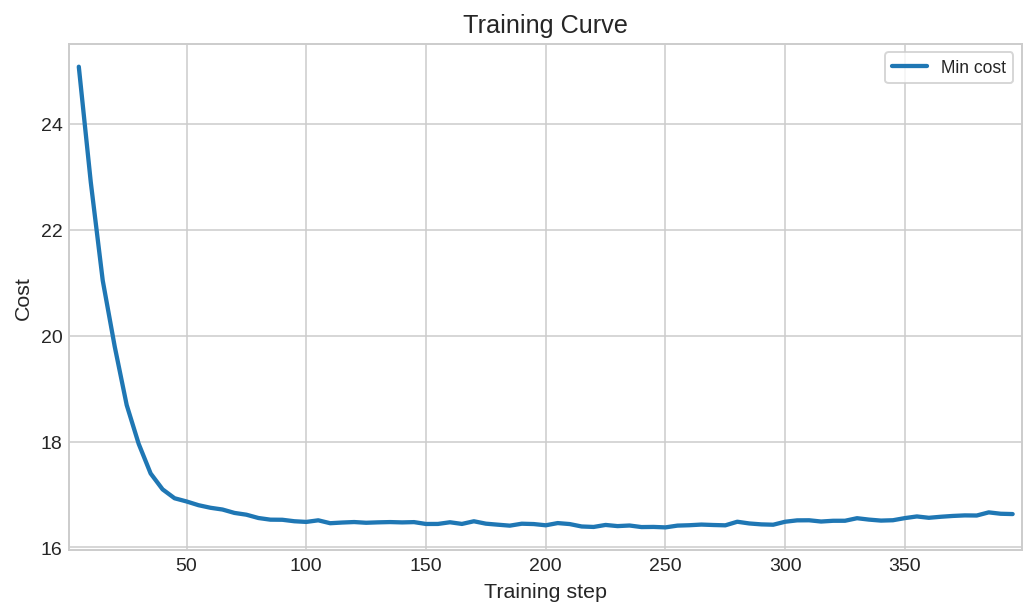
\includegraphics[width=\linewidth]{train_curv.png}
    \caption{Mean routing cost on the Nazari $N=100$ test set (1,000 instances) evaluated every 5 training epochs. The curve shows rapid initial learning followed by a convergence plateau around epoch 150.}
    \label{fig:training_curve}
\end{figure}

% ---------------------------------------------------------
% COMPONENT ABLATION
% ---------------------------------------------------------

\subsection{Local Search Heuristics and Feasibility Enforcement}
\label{sec:heuristics_feasibility}

Before analyzing the state representations, we first establish the optimal foundational search mechanics. We evaluated the interaction between three distinct local search heuristics (\textit{Insertion}, \textit{Swap}, and \textit{Two-Opt}) and three constraint-handling strategies:
\begin{itemize}
    \item \textbf{Indirect:} Allows intermediate infeasible states, relying on a greedy reconstruction to restore feasibility.
    \item \textbf{Proactive Filtering:} Explicitly masks invalid actions, ensuring the policy exclusively samples from the feasible subset.
    \item \textbf{Reactive Rejection:} Allows broader sampling but actively rejects or corrects moves that violate capacity constraints (e.g., via forced depot returns).
\end{itemize}

As shown in Table~\ref{tab:heuristic_feasibility}, no single constraint-handling strategy dominates across all heuristics; instead, performance is highly dependent on the pairing. 

\begin{table}[t]
\centering
\small
\caption{Cross-evaluation of Local Search Heuristics and Feasibility Enforcement Strategies on the Nazari $N=100$ test set ($10{,}000$ steps). Values represent Final Cost / Execution Time (s).}
\label{tab:heuristic_feasibility}
\begin{tabular}{l c c c}
\toprule
\textbf{Heuristic} & \textbf{Indirect} & \textbf{Proactive} & \textbf{Reactive} \\
\midrule
\textbf{Insertion} & 17.167 / 199.6s & \textbf{16.623} / 198.75s & 21.797 / 237.2s \\
\textbf{Swap} & 20.376 / 195.6s & 21.586 / 196.4s & 17.776 / 232.3s \\
\textbf{Two-Opt} & 21.339 / 204.9s & 18.990 / 334.1s & 18.131 / 237.6s \\
\bottomrule
\end{tabular}
\end{table}

The \textit{Insertion} heuristic combined with \textit{Proactive} filtering yields the absolute best performance, achieving a final cost of $16.623$ in $198.75$ seconds. By explicitly masking invalid insertion points, the policy efficiently navigates the feasible geometry without wasting compute on dead-end states. Conversely, pairing \textit{Insertion} with \textit{Reactive} rejection severely degrades the cost to $21.797$, as reactive corrections likely disrupt the fine-grained sequence improvements.

Interestingly, \textit{Swap} and \textit{Two-Opt} exhibit the opposite behavior: they perform poorly with proactive masking but achieve their best results under the \textit{Reactive} strategy ($17.776$ and $18.131$, respectively). However, because these alternative heuristic pairings still fall short of the \textit{Insertion + Valid} performance, we formally adopt the \textit{Insertion} heuristic with \textit{Proactive Filtering} as the standard algorithmic core for all subsequent architecture and feature evaluations.

\subsection{Feature Importance and Ablation Study}
\label{sec:feature_ablation}

To understand the contribution of individual state representations to the model's decision-making process, we conducted a comprehensive feature sweep. The features were categorized into topological variables, capacity variables, and spatial density metrics. We evaluated the architecture under three distinct protocols: Leave-One-Out (LOO) ablation, thematic grouping ablation, and isolated feature addition (where a minimal base model containing only static and meta features was supplemented with a single dynamic feature). All tests were evaluated on instances of $N=100$ for $10{,}000$ LG-SA steps.

\begin{table}[t]
\centering
\small
\setlength{\tabcolsep}{4pt}
\caption{Leave-One-Out (LOO) and Thematic Ablation Results. $\Delta$ Cost represents the degradation compared to the Baseline ($16.623$). Higher $\Delta$ implies higher feature importance.}
\label{tab:loo_ablation}
\begin{tabular}{l c c r}
\toprule
\textbf{Ablated Feature(s)} & \textbf{Final Cost} & \textbf{$\Delta$ Cost} & \textbf{Time (s)} \\
\midrule
\textbf{Baseline (All Features)} & \textbf{16.623} & -- & 198.75 \\
\midrule
\textit{Leave-One-Out Ablations} & & & \\
No Static & 21.600 & +4.977 & 156.41 \\
No Topology ($\mathbf{p}_{i-1}, \mathbf{p}_{i+1}$) & 17.201 & +0.578 & 170.90 \\
No Detour ($\Delta^{\text{detour}}_i$) & 17.154 & +0.531 & 182.19 \\
No Meta ($T, \tau$) & 16.862 & +0.239 & 181.83 \\
No Capacity Slack ($S_r$) & 16.702 & +0.079 & 188.30 \\
No Centroid Dist. ($d_{i, \text{cent}}$) & 16.660 & +0.037 & 185.67 \\
No Spatial Density ($\rho^{(33\%)}_i$) & 16.632 & +0.009 & 188.35 \\
No Spatial Density ($\rho^{(10\%)}_i$) & 16.604 & -0.019 & 188.33 \\
No Spatial Density ($\rho^{(5)}_i$) & 16.577 & -0.046 & 188.40 \\
No Node Load Ratio ($\eta_i$) & 16.562 & -0.061 & 188.27 \\
No Route Load Ratio ($L_r$) & \textbf{16.485} & \textbf{-0.138} & 193.24 \\
\midrule
\textit{Thematic Ablations} & & & \\
No Local Geometry$^*$ & 17.431 & +0.808 & 173.47 \\
No Capacity Status$^\dagger$ & 17.076 & +0.453 & 172.22 \\
No Spatial Density (All $\rho$) & 16.608 & -0.015 & 179.90 \\
\bottomrule
\multicolumn{4}{l}{\scriptsize $^*$ Excludes detour and centroid distance.} \\
\multicolumn{4}{l}{\scriptsize $^\dagger$ Excludes slack, route load ratio, and node load ratio.}
\end{tabular}
\end{table}

\paragraph{Critical Features (The Heavy Hitters)}
As expected, the \textit{Static} features (coordinates, polar angles, distance to depot, normalized demand) are strictly necessary; removing them leads to a catastrophic performance collapse (cost increases by $+4.977$). Beyond the static base, local geometric awareness is the primary driver of the model's success. Ablating the \textit{Topology} (neighbor coordinates) or the \textit{Detour} penalty degrades performance significantly ($+0.578$ and $+0.531$, respectively). This is further confirmed by the isolation experiments (Table~\ref{tab:isolation_ablation}): adding only \textit{Topology} to the minimal base model drops the cost from $20.112$ to $17.683$, and adding only \textit{Detour} drops it to $17.673$. The model heavily relies on immediate relational geometry to evaluate node insertions.

\paragraph{Moderate and Noisy Features}
Capacity-related features demonstrate mixed utility. While the thematic ablation of all capacity features degrades performance by $+0.453$, the LOO tests reveal that \textit{Capacity Slack} ($S_r$) is the most valuable individual capacity metric ($+0.079$ degradation when removed). Interestingly, ablating the \textit{Route Load Ratio} ($L_r$) actively \textit{improved} the final cost to $16.485$ (a $-0.138$ gain over the baseline). This suggests that $L_r$ may be introducing noise or redundancy that slightly misguides the model, indicating room for feature pruning.

\paragraph{Redundant Features}
The \textit{Spatial Density} metrics ($\rho^{(5)}, \rho^{(10\%)}, \rho^{(33\%)}$) appear almost entirely redundant. The thematic ablation of all three density features simultaneously resulted in a cost of $16.608$, which is statistically indistinguishable from the baseline ($16.623$). The isolation tests confirm this, as adding density features to the base model yielded negligible improvements (remaining trapped at costs $>20.0$). 

\begin{table}[t]

\centering

\small

\caption{Isolation Tests. Starting from a Base Model containing only \textit{Static} and \textit{Meta} features (Cost: $20.112$, Time: $113.49$s), individual features were added to isolate their independent value.}
\label{tab:isolation_ablation}
\begin{tabular}{l c r}
\toprule
\textbf{Isolated Feature Added} & \textbf{Final Cost} & \textbf{Time (s)} \\
\midrule
\textbf{Base Only (Static + Meta)} & \textbf{20.112} & 113.49 \\
\midrule
+ Detour ($\Delta^{\text{detour}}_i$) & 17.673 & 124.15 \\
+ Topology ($\mathbf{p}_{i-1}, \mathbf{p}_{i+1}$) & 17.683 & 130.44 \\
+ Centroid Dist. ($d_{i, \text{cent}}$) & 19.526 & 120.43 \\
+ Spatial Density ($\rho^{(10\%)}_i$) & 20.067 & 118.22 \\
+ Spatial Density ($\rho^{(33\%)}_i$) & 20.073 & 118.33 \\
+ Spatial Density ($\rho^{(5)}_i$) & 20.096 & 118.23 \\
+ Route Load Ratio ($L_r$) & 20.330 & 119.73 \\
+ Capacity Slack ($S_r$) & 20.562 & 119.65 \\
+ Node Load Ratio ($\eta_i$) & 20.591 & 119.71 \\
\bottomrule
\end{tabular}
\end{table}

\paragraph{Combinatorial Feature Pruning}
While ablating certain individual features---such as the Route Load Ratio ($L_r$) or specific Spatial Density metrics like ($\rho^{(5)}_i$)---yielded slight improvements or neutral effects compared to the baseline, combining these removals proved detrimental. We hypothesized that greedily stripping the architecture of all ``noisy'' or individually redundant features would yield a leaner, more accurate model. However, removing combinations of these features systematically degraded the solution quality, resulting in final costs exceeding $16.800$. This indicates that while some features may appear redundant in isolation, the model relies on a complex, non-linear interplay between them to maintain stability and guide the search space exploration effectively.

\paragraph{Computational Time Analysis}
Feature computation constitutes a significant portion of the total inference budget. The minimal base model executes in $113.49$ seconds, while the full baseline requires $198.75$ seconds, implying that dynamic feature extraction consumes roughly $43\%$ of the total runtime. 
Analyzing the Return on Compute Time (ROCT) provides a clear path for optimization. The \textit{Detour} feature is exceptionally efficient, yielding massive cost improvements for only an additional $\sim 10$ seconds of overhead in isolation. Conversely, the \textit{Spatial Density} features require nearly $19$ seconds to compute globally (as seen in the thematic density ablation: $198.75$s baseline vs. $179.90$s without density) but offer zero performance gain. By pruning the density metrics and potentially the noisy \textit{Route Load Ratio} feature, the model can achieve equal or better routing costs while significantly reducing inference times. Consequently, for all subsequent evaluations presented in this paper, we adopt the highest-performing architecture identified in this study—the optimized model trained without the \textit{Route Load Ratio} ($L_r$) feature—as our standard configuration.

\paragraph{Actor Network Architecture and Capacity}

To determine the optimal balance between computational efficiency and representational capacity, we evaluated three different network sizes by varying the embedding dimension and the number of hidden layers. Table~\ref{tab:architecture_comp} summarizes the performance and inference times for these configurations.

\begin{table}[t]
\centering
\small
\caption{Actor Network Architecture Comparison. Tests were evaluated over $10{,}000$ instances to measure the trade-off between network capacity, routing cost, and computation time.}
\label{tab:architecture_comp}
\begin{tabular}{c c c r}
\toprule
\textbf{Hidden Layers} & \textbf{Embedding Dim.} & \textbf{Final Cost} & \textbf{Time (s)} \\
\midrule
1 & 16 & 16.632 & 164.14 \\
\textbf{1} & \textbf{32} & \textbf{16.485} & \textbf{193.23} \\
2 & 32 & 16.516 & 229.13 \\
1 & 64 & 16.570 & 265.47 \\
\bottomrule
\end{tabular}
\end{table}

The empirical results clearly demonstrate that increasing the network's capacity is detrimental to both inference speed and solution quality. Expanding the depth (increasing hidden layers from $1$ to $2$) increased the computation time by roughly $18\%$ while slightly degrading the routing cost to $16.516$. Expanding the width (increasing the embedding dimension from $32$ to $64$) yielded the worst performance ($16.570$) and the highest computational overhead ($265.47$ seconds). 

These findings suggest that a highly parameterized network may overfit or struggle to maintain stable policy updates during the search process. Consequently, the minimal architecture---utilizing a single hidden layer and a 32-dimensional embedding---is not only the most computationally efficient but also provides the most effective gradient signals for the search process. This lean configuration is maintained as the default for all primary results.

\paragraph{Temperature Scheduling Strategy}

To optimize the Simulated Annealing (SA) process within our LG-SA framework, we evaluated two distinct temperature scheduling strategies to govern the exploration-exploitation tradeoff: a continuous exponential decay and a discrete step-wise decay. 

\begin{itemize}
    \item \textbf{Exponential Decay ($\alpha$ schedule):} This strategy smoothly reduces the temperature at each step using a continuous decay factor, defined as $\alpha = (T_\mathrm{final} / T_0)^{1/S}$, where $S$ is the total number of search steps.
    \item \textbf{Step Decay:} This strategy maintains a constant temperature for extended intervals, halving the temperature at specific epoch milestones (at 50\%, 66\%, 75\%, and roughly 85\% of the total steps) before abruptly dropping to $T_\mathrm{final}$ at the end of the schedule.
\end{itemize}

As detailed in Table~\ref{tab:temp_scheduling}, empirical evaluation demonstrated that the smooth, continuous cooling of the exponential decay schedule yielded superior results, achieving a final routing cost of $16.485$. In contrast, the discrete step decay converged to a slightly inferior cost of $16.519$. The continuous, granular adjustments of the exponential schedule likely allow the algorithm to traverse the search space and escape local optima more consistently than the abrupt, discrete transitions of the step schedule.

\begin{table}[t]
\centering
\small
\caption{Comparison of Simulated Annealing Temperature Scheduling Strategies. Both strategies were evaluated using the optimized model configuration.}
\label{tab:temp_scheduling}
\begin{tabular}{l c}
\toprule
\textbf{Scheduling Strategy} & \textbf{Final Cost} \\
\midrule
\textbf{Exponential Decay ($\alpha$)} & \textbf{16.485} \\
Step Decay & 16.519 \\
\bottomrule
\end{tabular}
\end{table}


\paragraph{Critic Architecture}
We compare two value-function architectures. The \textit{FF Critic} applies an MLP to each node independently and aggregates via mean pooling — computationally cheap but treating node contributions as additive. The \textit{Attention Critic} instead uses multi-head attention pooling with a learnable query vector, allowing the network to weight nodes by geometric relevance. Using our optimized feature set and the \textit{Immediate} reward, the FF Critic achieves a final cost of $16.485$ versus $16.713$ for the Attention variant. The added capacity of attention pooling does not compensate for its training instability at this scale, so we adopt the FF Critic for all subsequent experiments.

\subsection{Reward Signal Formulation}
\label{sec:reward_formulation}

The reward $r_t$ encodes move quality for the PPO agent at each SA step. The two base designs are the \textit{Immediate} formulation — a tiered signal based on action outcome:
\begin{equation}
    r_t = \begin{cases} -1.5 & \text{invalid move} \\ 0 & \text{valid but SA-rejected} \\ C(s_t) - C(s_{t+1}) & \text{accepted} \end{cases}
\end{equation}
(normalized by $C(s_0)$); and the \textit{Global Best} formulation, which gives a sparse reward tied only to strict improvements over the historical best $s^*_t$:
\begin{equation}
    r_t^{\text{GB}} = \max\!\big(0,\, C(s^*_t) - C(s_{t+1})\big).
\end{equation}
Beyond these two anchors, we evaluate nine total formulations grouped into four families:
\begin{itemize}
    \item \textbf{Immediate/Dense Rewards:} Provide granular feedback at every step based on the actual change in routing cost ($\Delta_{\text{actual}}$). The \textit{Immediate} strategy directly rewards positive improvements. The \textit{SA-Aligned} variant mirrors the Simulated Annealing logic, selectively penalizing rejected moves ($-0.1$).
    \item \textbf{Global/Sparse Rewards:} Tie the reward to the discovery of new global best solutions. The \textit{Global Best} strategy grants a normalized reward only when the historical best cost is strictly improved, treating all other steps as zero-reward transitions. The \textit{Terminal} strategy is maximally sparse, withholding all feedback until the final step $T$, where it evaluates the total percentage improvement relative to the initial cost.
    \item \textbf{Curriculum and Hybrid Strategies:} Attempt to balance short-term guidance with long-term optimality. \textit{Hybrid} uses a static linear combination ($\alpha = 0.5$) of the \textit{Immediate} and \textit{Global Best} signals. The \textit{Curriculum} approaches dynamically shift the reward signal across epochs, linearly transitioning from \textit{SA-Aligned} dense rewards early in training to either \textit{Global Best} or \textit{Terminal} rewards in the final epochs (evaluated over $250$ epochs).
    \item \textbf{Step Penalties:} Impose a continuous negative penalty at each step proportional to the current trajectory cost, scaled either by the initial cost (\textit{Step Penalty Init}) or an arbitrary theoretical baseline (\textit{Step Penalty 16}), encouraging the agent to minimize the route length purely to reduce the accumulated step penalties.
\end{itemize}

The models were evaluated under identical inference conditions ($N=100$, $10{,}000$ search steps). Results are summarized in Table~\ref{tab:reward_formulations}.

\begin{table}[t]
\centering
\small
\caption{Performance comparison of PPO reward formulations on the Nazari $N=100$ test set over $10{,}000$ steps. Cost are averaged over the benchmark.}
\label{tab:reward_formulations}
\begin{tabular}{l c}
\toprule
\textbf{Reward Strategy} & \textbf{Final Cost}\\
\midrule
\textbf{Immediate} & \textbf{16.485} \\
Curriculum Terminal & 16.547 \\
Curriculum (SA $\to$ Global) & 16.573  \\
SA-Aligned & 16.582  \\
Global Best & 16.604  \\
Hybrid (Immediate + Global) & 16.632  \\
Terminal & 17.498 \\
Step Penalty Init & 29.989  \\
Step Penalty 16 & 30.341 \\
\bottomrule
\end{tabular}
\end{table}

\paragraph{Dense Signals Dominate}
The empirical results clearly indicate that the PPO agent thrives on dense, highly localized feedback. The \textit{Immediate} reward formulation achieved the absolute best routing cost of $16.485$. By providing a clear, normalized gradient of improvement at every individual step, the agent can correctly attribute value to specific local geometric transformations, a necessity for fine-grained routing improvements. The closely related \textit{SA-Aligned} strategy also performed well ($16.582$), though explicitly penalizing rejected moves appears slightly less optimal than the pure, symmetric feedback of actual cost variations.

\paragraph{The Cost of Sparsity}
As the reward signal becomes sparser, solution quality degrades. Relying solely on the \textit{Global Best} improvements yielded a cost of $16.604$, as the agent likely suffers from the credit assignment problem during extended plateaus where no new global best is found. This degradation is most pronounced in the \textit{Terminal} setting ($17.498$), proving that evaluating a step sequence strictly by its final outcome provides insufficient gradient resolution for the policy to learn complex insertion heuristics.

\paragraph{Curriculum Approaches}
Interestingly, the \textit{Curriculum Terminal} ($16.547$) and standard \textit{Curriculum} ($16.573$) strategies offered very strong performance, nearly matching the baseline \textit{Immediate} approach. Transitioning the agent from dense, local guidance to global, objective-oriented rewards effectively leverages the benefits of both paradigms. However, because these methods introduce additional hyperparameter complexity without surpassing the straightforward \textit{Immediate} formulation, we maintain the \textit{Immediate} reward signal as the optimal default.

\paragraph{Failure of Step Penalties}
Finally, the \textit{Step Penalty} frameworks failed catastrophically, collapsing to costs near $30.0$. Continuous negative rewards per step fundamentally clash with the mechanics of the routing problem, likely inducing premature convergence or erratic policy updates as the agent attempts to ``escape'' the environment rather than systematically optimizing the topological sequences.

These results highlight the critical importance of reward density. The model trained with the \textit{Immediate} formulation ($16.485$) significantly outperforms the model trained with the \textit{Global Best} formulation ($16.604$), a gap of $0.119$ routing units. This confirms that sparse, trajectory-level feedback is insufficient for our local search paradigm: the dense, step-by-step gradient provided by the immediate improvement signal allows the agent to accurately map the granular contours of the cost landscape, enabling deeper convergence.

\paragraph{Impact of the Metropolis Criterion}
We assessed the contribution of the stochastic Metropolis acceptance criterion during both the training and inference phases (Table~\ref{tab:metropolis_ablation}). The evaluation reveals that stochasticity is highly beneficial across the entire pipeline. 

Employing the Metropolis criterion during \textit{testing} consistently yields superior results, improving the final cost by approximately $0.11$ to $0.16$ regardless of the training method ($16.485$ vs. $16.652$ for the Metropolis-trained model, and $16.567$ vs. $16.684$ for the Descent-trained model). This confirms its expected role in allowing the search process to escape shallow local minima at inference time.

More importantly, we observe that employing the Metropolis criterion during \textit{training} acts as a crucial regularizer. The model trained with Metropolis outperforms the strict Descent-trained model in all test scenarios. Specifically, when both models are evaluated using the optimal Metropolis testing criterion, the Metropolis-trained model achieves the global best cost of $16.485$ versus $16.567$ for the descent-trained baseline. This indicates that the stochasticity introduced during training prevents the model from overfitting to specific greedy descent trajectories, resulting in a more generalized and robust value estimation.

\begin{table}[t]
\centering
\small
\caption{Impact of the Metropolis Criterion (Train vs. Test). Evaluated on instances of $N=100$ for $10{,}000$ LG-SA steps.}
\label{tab:metropolis_ablation}
\begin{tabular}{l c c c}
\toprule
\textbf{Train Criterion} & \textbf{Test Criterion} & \textbf{Final Cost} \\
\midrule
\textbf{Metropolis} & \textbf{Metropolis} & \textbf{16.485} \\
Metropolis & Descent & 16.652 \\
\midrule
Descent & Metropolis & 16.567 \\
Descent & Descent  & 16.684 \\
\bottomrule
\end{tabular}
\end{table}

% ---------------------------------------------------------
% ROBUSTNESS / GENERALIZATION
% ---------------------------------------------------------
\subsection{Robustness and Generalization}

\paragraph{Initialization Sensitivity}
We investigated how the choice of training initialization impacts the model's ability to generalize to unseen starting conditions (Table~\ref{tab:init_generalization}). To thoroughly evaluate this, we tested the models across a wide spectrum of initial states: ranging from highly unoptimized configurations (\textit{Isolate} — each customer placed in its own single-node route, yielding a severe initial cost of $104.045$) to greedy heuristic constructions (\textit{Nearest Neighbor}, starting at a highly optimized $18.989$).

Surprisingly, the model trained exclusively on \textit{Random} initialization demonstrated superior performance and remarkable robustness across \textit{all} test scenarios. It consistently converged to a final cost between $16.46$ and $16.53$, regardless of whether the initial trajectory was near-optimal or pathologically poor. Remarkably, it achieved its absolute best final cost ($16.468$) when starting from the absolute worst initialization (\textit{Isolate}). 

In contrast, models trained specifically on structured heuristics (\textit{Sweep}, \textit{Nearest Neighbor}) or extreme distributions (\textit{Isolate}) failed catastrophically when applied to out-of-distribution initial states. More importantly, they were vastly outperformed by the \textit{Random} model even on their own specialized test sets. The \textit{Multi-init} approach, intended to provide exposure to varied starting points, performed moderately well but still failed to match the convergence of pure random training. These results strongly suggest that the high variance and lack of structural bias inherent in random initialization act as a powerful regularizer. It forces the model to learn a comprehensive, global representation of the cost landscape rather than overfitting to the narrow descent trajectories of specific constructive heuristics.

\begin{table}[t]
\centering
\small
\caption{Cross-Initialization Performance ($N=100$, 10k steps). Each model was trained on a specific initial state distribution and tested across four distinct initialization types.}
\label{tab:init_generalization}
\begin{tabular}{l l r c}
\toprule
\textbf{Train Init} & \textbf{Test Init} & \textbf{Init Cost} & \textbf{Final Cost} \\
\midrule
\textbf{Random} & Random & 57.830 & \textbf{16.485} \\
Multi-init & Random & 57.830 & 17.012 \\
Sweep & Random & 57.830 & 18.556 \\
Nearest Neighbor & Random & 57.830 & 20.356 \\
Isolate & Random & 57.830 & 21.106 \\
\midrule
\textbf{Random} & Sweep  & 30.458 & \textbf{16.488} \\
Multi-init & Sweep  & 30.458 & 16.992 \\
Sweep & Sweep  & 30.458 & 17.309 \\
Isolate & Sweep  & 30.458 & 18.039 \\
Nearest Neighbor & Sweep  & 30.458 & 19.048 \\
\midrule
\textbf{Random} & Nearest Neighbor & 18.989 & \textbf{16.531} \\
Multi-init & Nearest Neighbor & 18.989 & 17.056 \\
Sweep & Nearest Neighbor & 18.989 &  17.154 \\
Isolate & Nearest Neighbor & 18.989 & 17.891 \\
Nearest Neighbor & Nearest Neighbor & 18.989 & 18.424 \\
\midrule
\textbf{Random} & Isolate & 104.045 & \textbf{16.468} \\
Multi-init & Isolate & 104.045 & 16.973 \\
Sweep & Isolate & 104.045 & 17.388 \\
Isolate & Isolate & 104.045 & 17.447 \\
Nearest Neighbor & Isolate & 104.045 & 20.376 \\
\bottomrule
\end{tabular}
\end{table}

\paragraph{Cross-Distribution Generalization}
Table~\ref{tab:data_generalization} illustrates the generalization capabilities of our architecture across different problem topologies. We compared our optimal model trained on the uniform Random distribution \citep{nazari_reinforcement_2018} against a model trained exclusively on the structurally diverse, complex topologies generated by the \citet{queiroga_10000_nodate} script.

The empirical results reveal a striking dominance of the Random-trained model. As expected, it drastically outperforms the Queiroga-trained model on the uniform Random test set ($16.485$ vs. $16.921$). However, the most significant finding is that the Random-trained model also \textit{outperforms the specialist model on its own target distribution}, achieving a final cost of $19.727$ on the Queiroga test set compared to the specialist's $19.891$. 

This reinforces a core conclusion regarding our neural architecture: introducing extreme structural complexity during training (as found in the Queiroga instances) actually hinders the model's ability to learn efficient, generalized descent trajectories. Instead, training on simple, uniform random distributions provides an unbiased baseline that forces the network to learn the fundamental spatial and capacity mechanics of the CVRP, yielding a highly robust model capable of tackling complex, clustered topologies zero-shot.

\begin{table}[t]
\centering
\small
\caption{Cross-Distribution Generalization ($N=100$). Evaluated for $10{,}000$ LG-SA steps.}
\label{tab:data_generalization}
\begin{tabular}{l l c c}
\toprule
\textbf{Train Dist.} & \textbf{Test Dist.} & \textbf{Init Cost} & \textbf{Final Cost} \\
\midrule
\textbf{Random} & Random & 57.830 & \textbf{16.485} \\
Queiroga & Random & 57.830 & 16.921 \\
\midrule
\textbf{Random} & Queiroga & 57.983 & \textbf{19.727} \\
Queiroga & Queiroga & 57.983 & 19.891 \\
\bottomrule
\end{tabular}
\end{table}

% ---------------------------------------------------------
% CURRICULUM LEARNING
% ---------------------------------------------------------
\paragraph{Curriculum Learning and Catastrophic Forgetting}
Rather than always training from purely random initializations, we progressively pre-improve starting states by running the current policy for $T_{\text{init}}$ steps before each PPO update. Following \citet{ma_learning_2021}, $T_{\text{init}}$ grows via a sigmoid schedule:
\begin{equation}
    T_{\text{init}} = \frac{S(e) - S(0)}{S(E) - S(0)} \xi_{\text{CL}},
\end{equation}
where $e$ is the current epoch, $E$ the total number of epochs, $\xi_{\text{CL}}$ the maximum curriculum depth, and $S(x) = \bigl(1 + e^{-\kappa x}\bigr)^{-1}$ is the logistic sigmoid with steepness $\kappa$. This forces the agent to learn on already-optimized states, but risks catastrophic forgetting if depth is too large. We evaluated the effect of $\xi_{\text{CL}}$ and schedule shape (Linear vs.\ Sigmoid with steepness $\kappa$).

Notably, an extreme depth of $\xi_{\text{CL}} = 2500$ was previously identified as optimal for heavyweight constructive policies like DACT \citep{ma_learning_2021}. However, as shown in Table~\ref{tab:curriculum_learning}, applying this depth to our local search architecture severely degraded performance ($17.081$). Because our lightweight model must accurately estimate the value of local moves across the entire cost landscape, pushing the training distribution too deep into local minima induces catastrophic forgetting of the chaotic, unoptimized ``early game.'' 

Our comprehensive sweep over a standard 200-epoch horizon reveals that a shallow maximum depth of $\xi_{\text{CL}} = 200$ steps acts as a hard architectural threshold. Within this optimal depth, an ultra-flat Sigmoid schedule ($\kappa=0.01$) achieved a highly competitive final cost of $16.430$. Interestingly, this peak performance was not obtained at the very end of training, but rather near the midpoint (epoch 110), corresponding precisely to $T_{\text{init}} = 110$. After this point, performance began to slowly degrade as the curriculum pushed deeper.

This observation led to a critical hypothesis: the network possesses a structural ``sweet spot'' at around $T_{\text{init}} = 110\text{--}120$, where it perfectly balances structural optimization without losing global landscape awareness. To test this, we evaluated an extended 1000-epoch training horizon, slowing down the curriculum to allow the model extensive training within this optimal pre-step threshold. We tested this extended horizon across a Linear schedule, a steeper Sigmoid ($\kappa=0.02$), and the ultra-flat Sigmoid ($\kappa=0.01$) with maximum curriculum depths of both $\xi_{\text{CL}} = 200$ and $\xi_{\text{CL}} = 500$. 

As predicted, expanding the horizon yielded massive breakthroughs across the board, with all configurations outperforming the 200-epoch baseline. The $\xi_{\text{CL}} = 200$ configurations showed excellent consistency, all achieving final costs tightly clustered between $16.370$ and $16.389$. However, expanding the depth to $\xi_{\text{CL}} = 500$ with the ultra-flat Sigmoid ($\kappa=0.01$) ultimately reached a new global best final cost of $\textbf{16.343}$. Crucially, this champion checkpoint emerged exactly at epoch 250, corresponding to $T_{\text{init}} = 120$ pre-steps. This confirms that for lightweight local search critics, identifying and maximizing exposure to this moderate structural threshold is far superior to standard deep-curriculum approaches.

\begin{table}[t]
\centering
\small
\caption{Impact of Curriculum Learning configurations. Evaluated on $N=100$ for $10{,}000$ LG-SA steps.}
\label{tab:curriculum_learning}
\begin{tabular}{l c c c r}
\toprule
\textbf{Schedule} & \textbf{\shortstack{Steepness \\ ($\kappa$)}} & \textbf{\shortstack{Max Steps \\ ($\xi_{\text{CL}}$)}} & \textbf{Final Cost} & \textbf{Gap} \\
\midrule
None (Baseline)& -- & 0 & 16.485 & -- \\
\midrule
\multicolumn{5}{l}{\textit{Standard Horizon (200 Epochs)}} \\
Sigmoid & 0.01 & 200 & 16.430 & -0.055 \\
Linear & -- & 200 & 16.454 & -0.031 \\
Sigmoid & 0.02 & 200 & 16.470 & -0.015 \\
Sigmoid & 0.02 & 500 & 16.509 & +0.024 \\
Linear & -- & 500 & 16.592 & +0.107 \\
Sigmoid & 0.01 & 500 & 16.633 & +0.148 \\
Sigmoid & 0.02 & 2,500 & 17.081 & +0.596 \\
\midrule
\multicolumn{5}{l}{\textit{Extended Horizon (1000 Epochs)}} \\
Sigmoid & 0.02 & 200 & 16.370 & -0.115 \\
Linear & -- & 200 & 16.376 & -0.109 \\
Sigmoid & 0.01 & 200 & 16.389 & -0.096 \\
Sigmoid & 0.02 & 500 & 16.393 & -0.092 \\
Linear & -- & 500 & 16.404 & -0.081 \\
Sigmoid & 0.01 & 500 & \textbf{16.343} & \textbf{-0.142} \\
\bottomrule
\end{tabular}
\end{table}

% ---------------------------------------------------------
% SCALING
% ---------------------------------------------------------
\subsection{Scalability Analysis}
We conducted a comprehensive scaling analysis across problem dimensions $N=10$ to $N=100$ and search durations up to $200{,}000$ steps. As detailed in Table~\ref{tab:scaling_results} and visualized in Figure~\ref{fig:scaling_plots_full}, the method exhibits a consistent logarithmic convergence profile.
For $N=100$, increasing the budget from $100$ to $10{,}000$ steps yields a massive $32.0\%$ reduction in cost ($24.046 \to 16.343$). Diminishing returns appear thereafter; extending the search to $100{,}000$ steps yields only a $2.2\%$ further improvement ($16.343 \to 15.985$). Runtime scales linearly with steps and polynomially with dimension, confirming computational tractability even for extended search horizons.

\begin{table}[t]
\centering
\small
\caption{Scaling Analysis: Cost and Time vs. Steps and Dimension.}
\label{tab:scaling_results}
\begin{tabular}{c r c c}
\toprule
\textbf{Dim ($N$)} & \textbf{Steps} & \textbf{Cost} & \textbf{Time (s)} \\
\midrule
\multirow{6}{*}{10} 
  & 100     & 4.804 & 0.22 \\
  & 1,000   & 4.631 & 1.61 \\
  & 5,000   & 4.574 & 7.87 \\
  & 10,000  & 4.558 & 15.72 \\
  & 100,000 & 4.532 & 158.05 \\
  & 200,000 & 4.528 & 319.39 \\
\midrule
\multirow{6}{*}{20}
  & 100     & 6.715 & 0.36 \\
  & 1,000   & 6.339 & 3.18 \\
  & 5,000   & 6.233 & 15.69 \\
  & 10,000  & 6.204 & 31.49 \\
  & 100,000 & 6.144 & 313.63 \\
  & 200,000 & 6.135 & 627.98 \\
\midrule
\multirow{6}{*}{50} 
  & 100     & 12.689 & 0.99 \\
  & 1,000   & 11.082 & 9.38 \\
  & 5,000   & 10.760 & 46.70 \\
  & 10,000  & 10.676 & 93.21 \\
  & 100,000 & 10.503 & 933.19 \\
  & 200,000 & 10.472 & 1867.44 \\
  & 500,000 & 10.437 & 4357.86 \\
  & 1,000,000 & 10.418 & 8718.43 \\
\midrule
\multirow{6}{*}{100} 
  & 100     & 24.046 & 2.01 \\
  & 1,000   & 17.316 & 19.61 \\
  & 5,000   & 16.528 & 97.85 \\
  & 10,000  & 16.343 & 193.89 \\
  & 100,000 & 15.985 & 1899.76 \\
  & 200,000 & 15.918 & 3781.67 \\
  & 500,000 & 15.850 & 8136.74 \\
  & 1,000,000 & 15.809 & 16236.13 \\
\bottomrule
\end{tabular}
\end{table}

\begin{figure*}[t!]
    \centering
    \begin{subfigure}[b]{0.48\textwidth}
        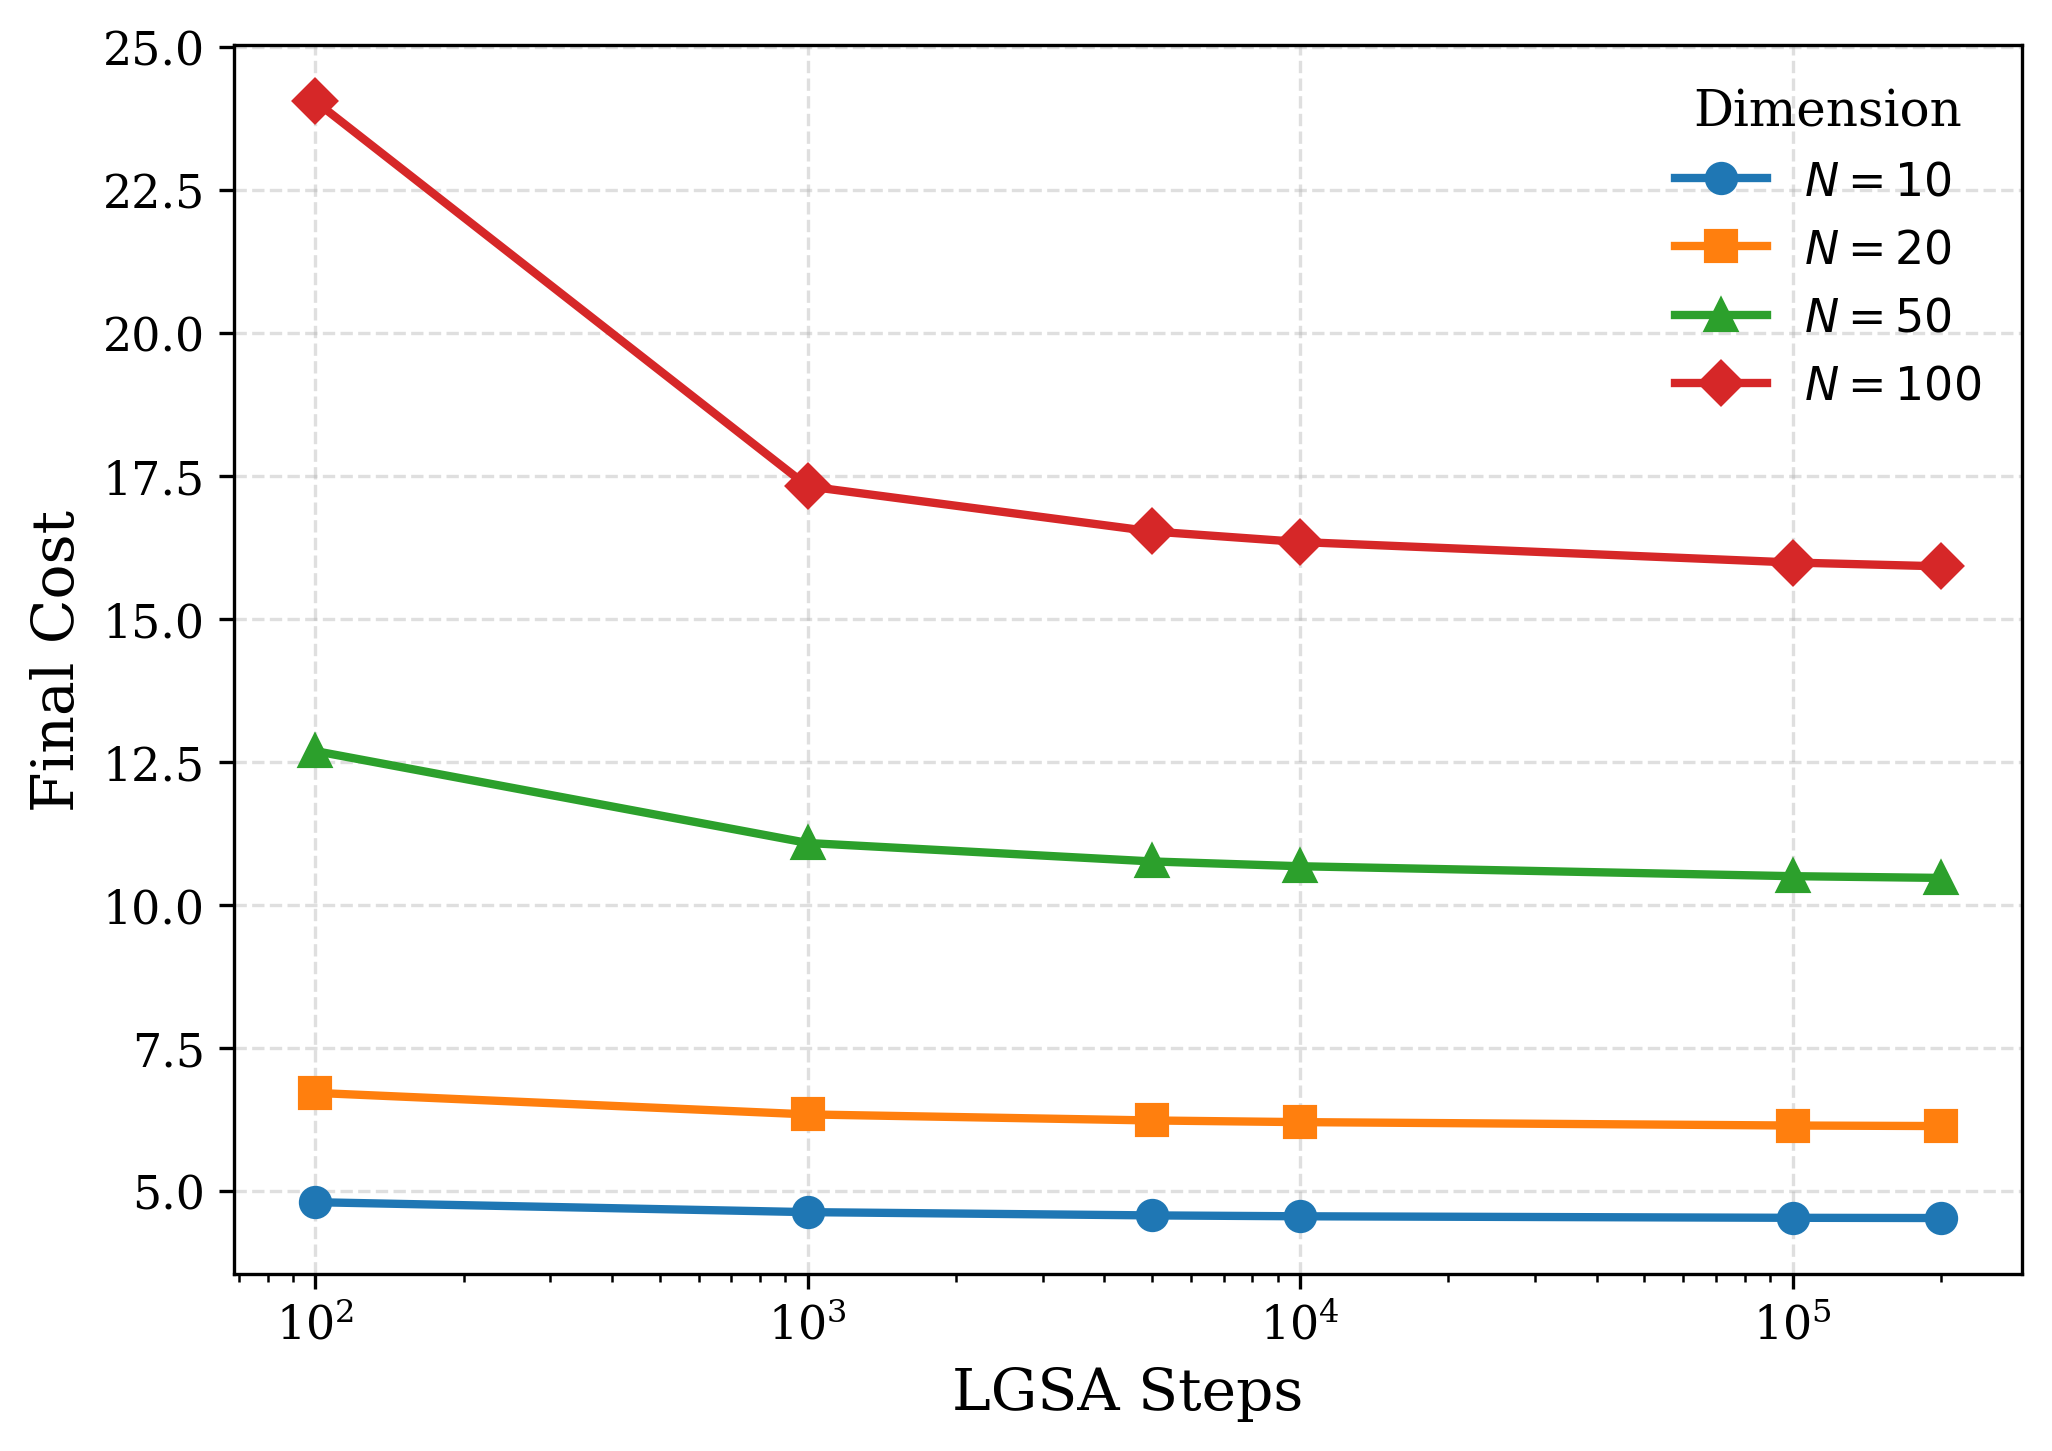
\includegraphics[width=\linewidth]{res.png}
        \caption{\textbf{Convergence of Final Cost.}}
        \label{fig:res}
    \end{subfigure}
    \hfill
    \begin{subfigure}[b]{0.48\textwidth}
        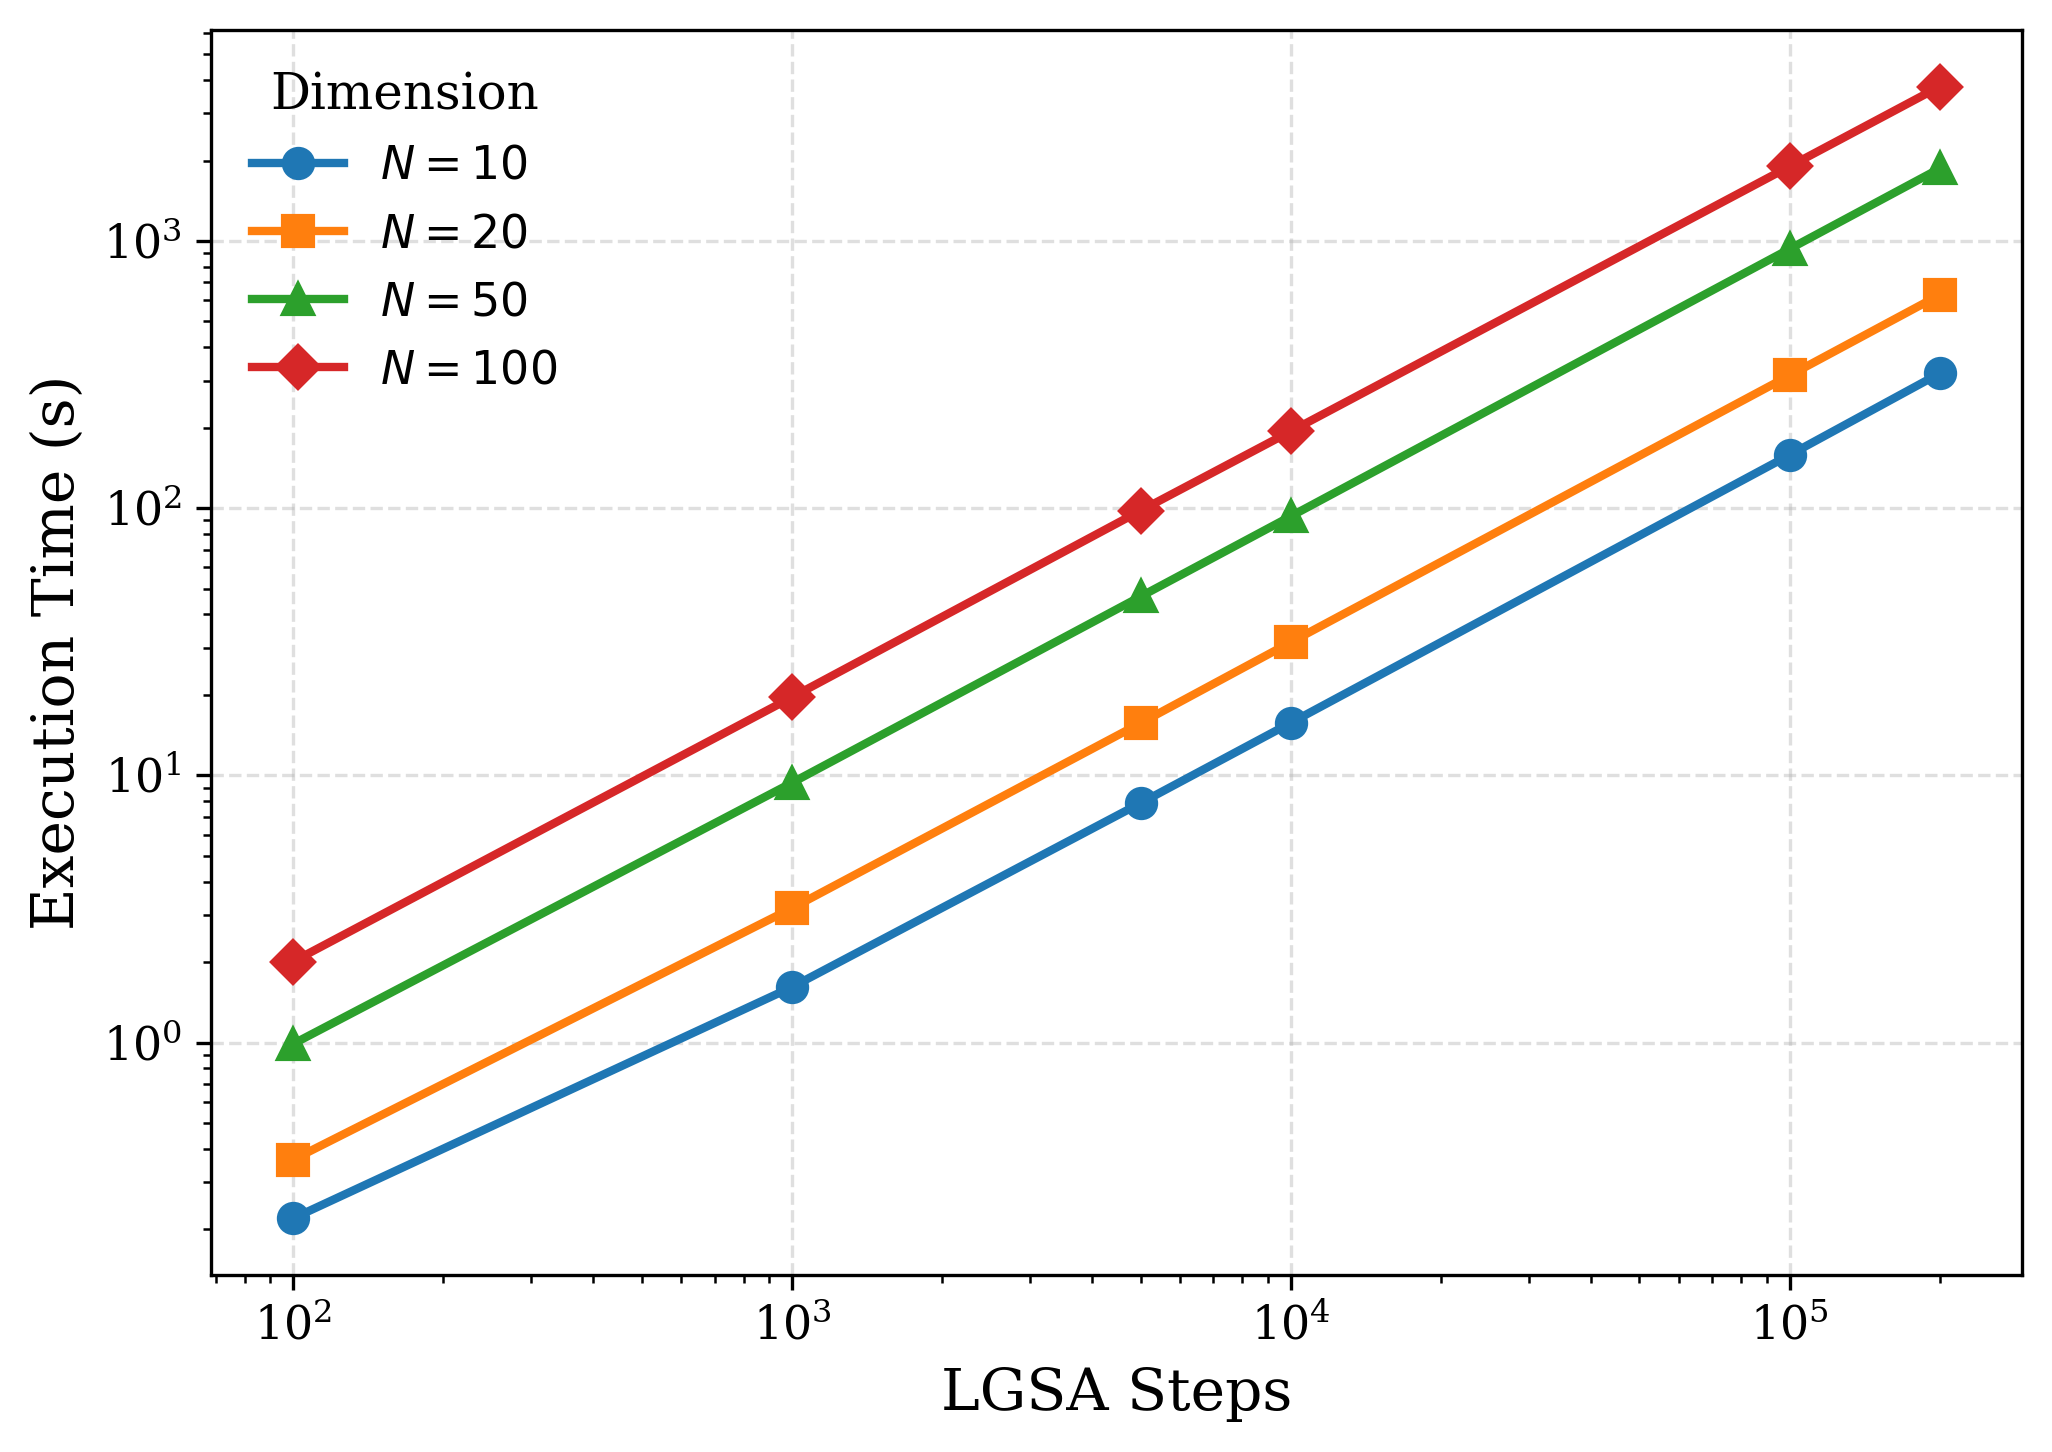
\includegraphics[width=\linewidth]{time.png}
        \caption{\textbf{Execution Time Scaling.}}
        \label{fig:time}
    \end{subfigure}
    \caption{Scaling Analysis. (a) Evolution of solution quality as a function of LG-SA steps across problem dimensions. (b) Computational time scaling with respect to steps and problem size (log-log scale).}
    \label{fig:scaling_plots_full}
\end{figure*}

\paragraph{Extreme-Scale Dimension Scaling}
Beyond standard benchmark dimensions, we also evaluated the model's execution time scaling for massive instances. To isolate the computational complexity of the search process itself, this evaluation was performed sequentially on a CPU, processing instances one by one. Figure~\ref{fig:time_nodes} illustrates the wall-clock time required to process graphs scaling from standard sizes up to extreme-scale environments of $N=10{,}000$ nodes, evaluated under fixed budgets of $1{,}000$ and $10{,}000$ steps. 

The empirical results demonstrate highly efficient, near-linear computational scaling with respect to the problem dimension. For a budget of $1{,}000$ steps, execution times remain remarkably low, averaging $1.06$ seconds across the evaluated sizes and peaking at just $3.15$ seconds for the largest $10{,}000$-node graph. When extending the search horizon to $10{,}000$ steps, the execution time scales proportionally, yielding a mean of $10.57$ seconds and a maximum of $31.87$ seconds for the extreme-scale instance. This stable and predictable computational profile confirms the method's exceptional architectural tractability and its practical suitability for massive real-world routing scenarios.

\begin{figure}[t]
    \centering
    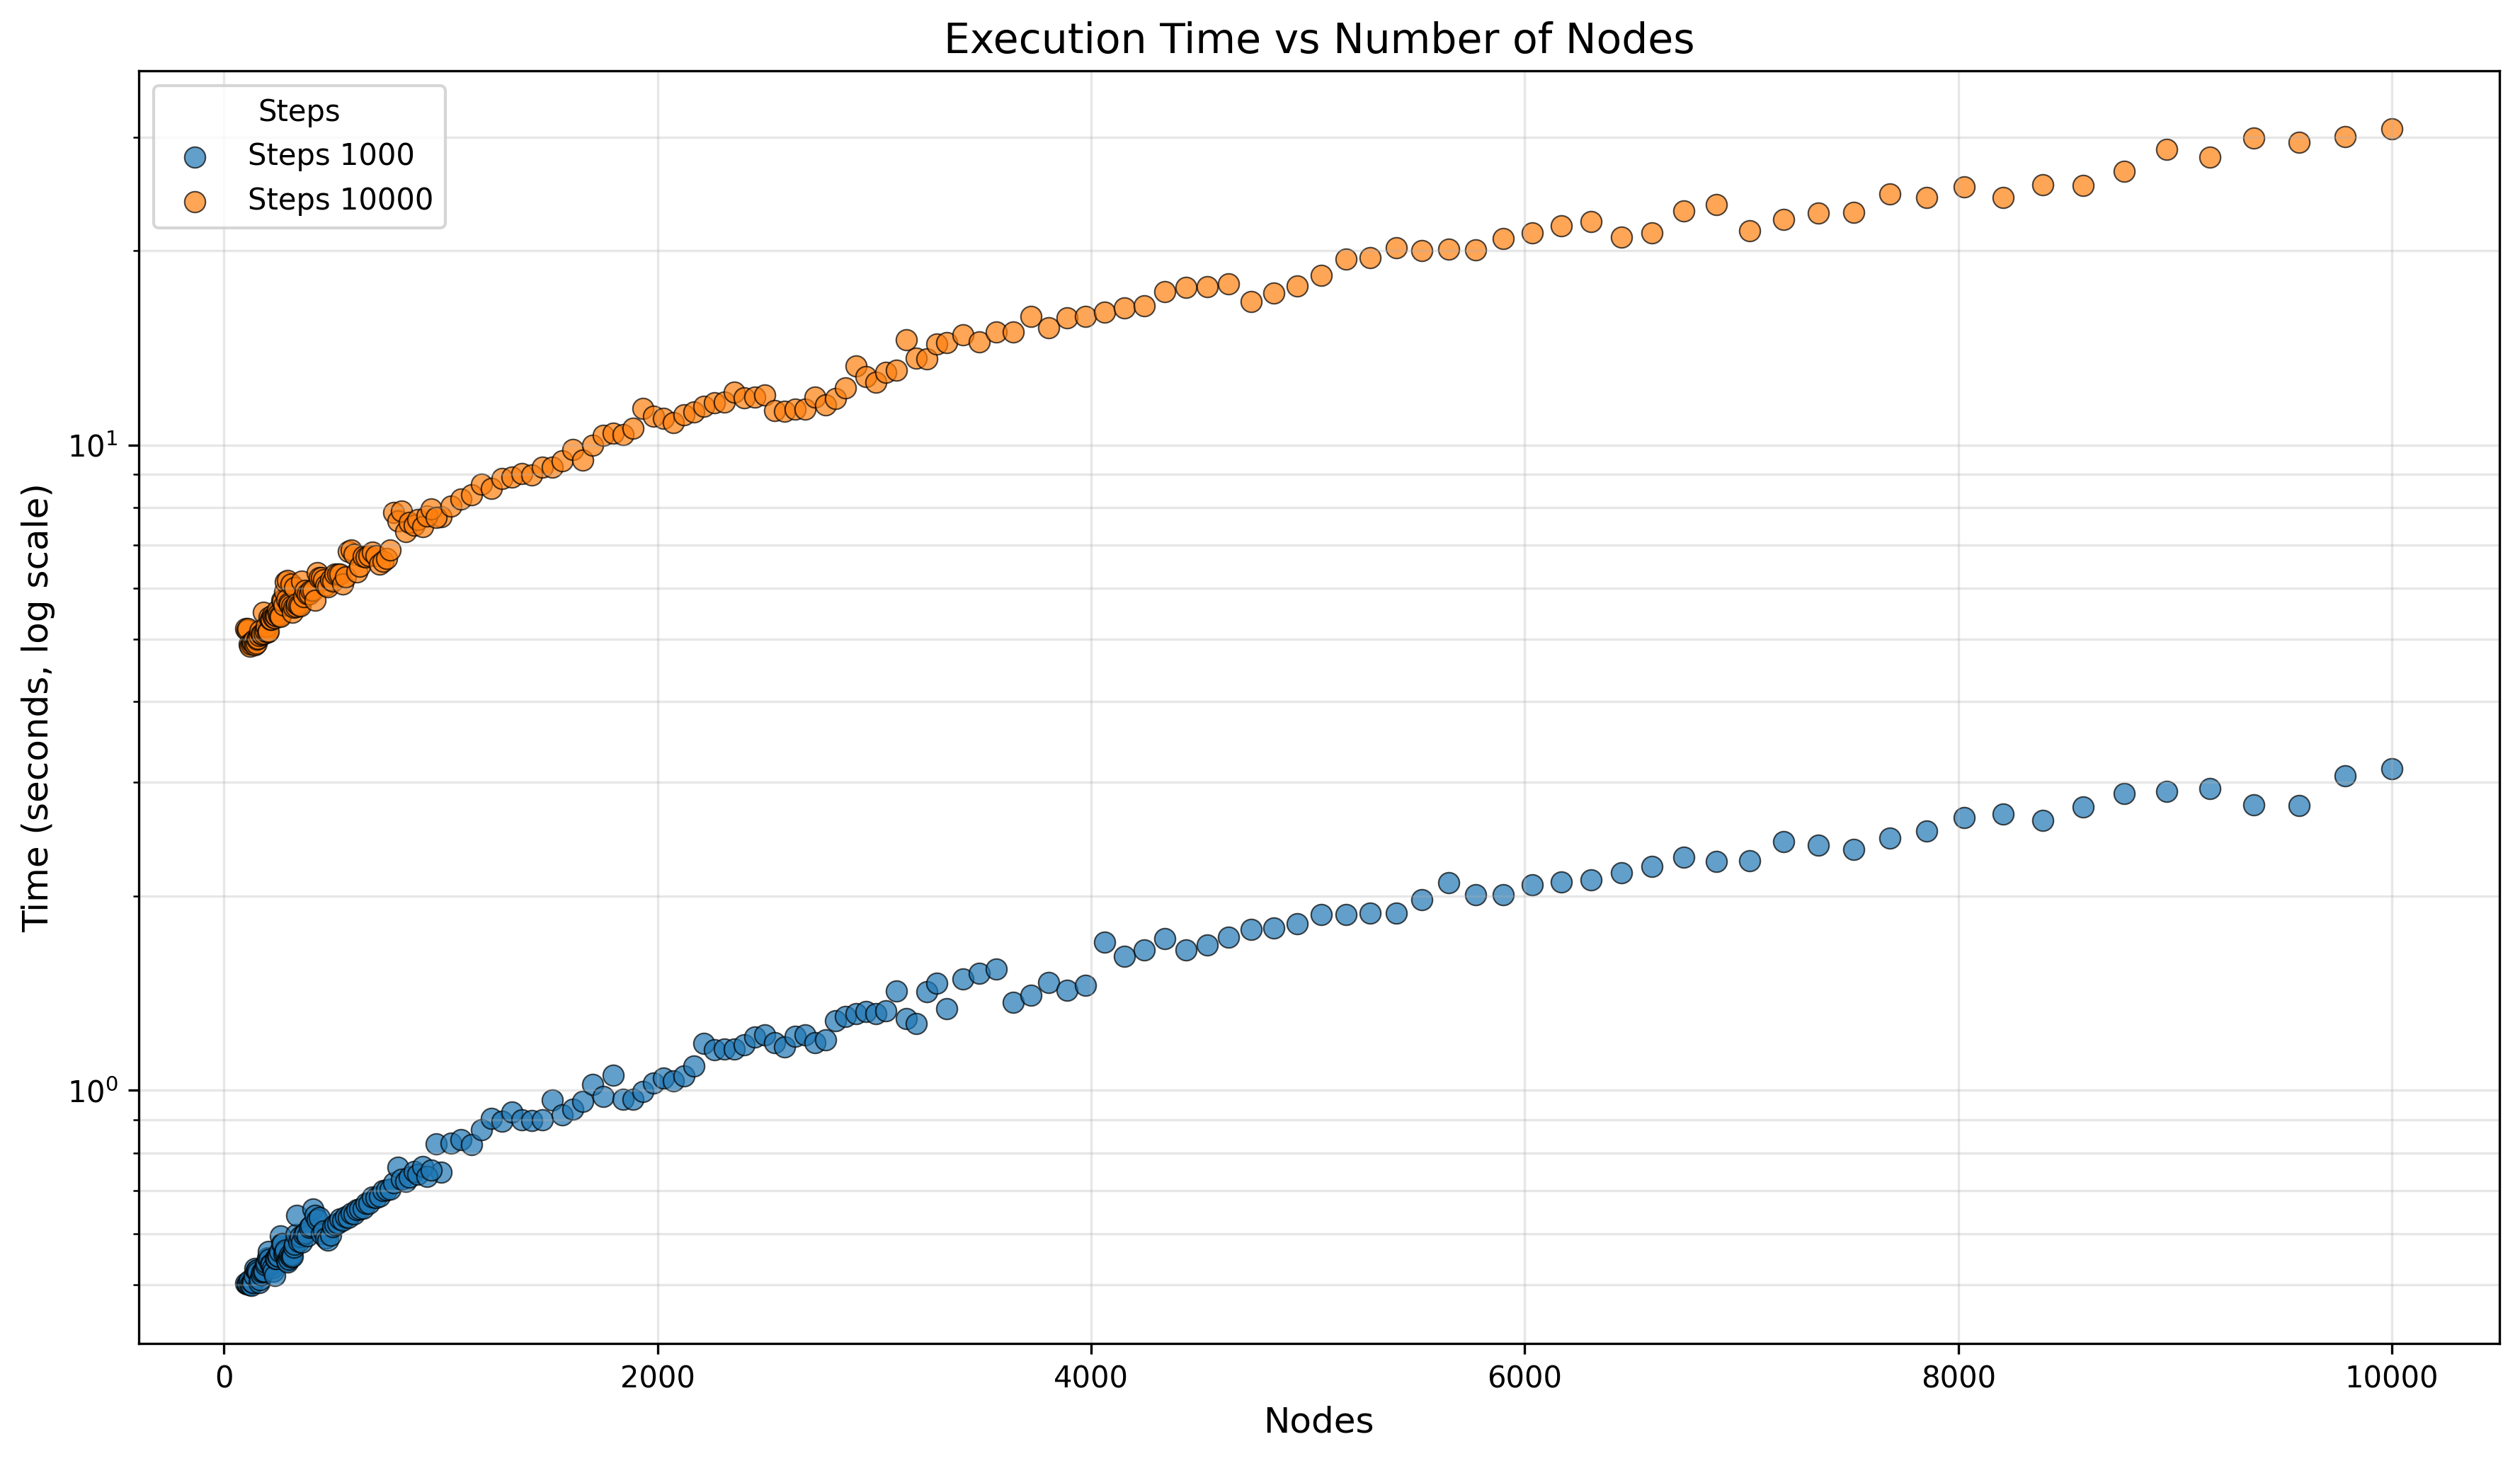
\includegraphics[width=\linewidth]{time_nodes.png}
    \caption{Sequential CPU execution time (in seconds) as a function of problem dimension ($N$). The model exhibits near-linear scaling, maintaining extreme efficiency for both $1{,}000$ and $10{,}000$ step budgets on massive instances up to $N=10{,}000$.}
    \label{fig:time_nodes}
\end{figure}

\paragraph{Parallelization and Batch Scaling}
To quantify the efficiency of our batched evaluation on GPU, we analyzed the impact of the batch size (number of parallel instances) on the total execution time. This test was performed on instances of dimension $N=100$, executing a fixed budget of $10{,}000$ LG-SA steps. The results in Table~\ref{tab:batch_scaling} reveal a distinct three-phase scaling regime. 

For small batches (100 to $1{,}000$ instances), increasing the workload by a factor of 10 only increases the execution time marginally (from $11.01$ s to $15.27$ s). In this regime, the GPU is under-saturated, and the constant overhead of kernel launches dominates. Peak hardware efficiency is observed between $1{,}000$ and $2{,}000$ instances, where the GPU compute capacity is optimally saturated, bringing the time per instance down to a minimum of $\sim 15.2$ ms. Beyond $2{,}000$ instances, the hardware enters a memory-bound state, and the execution time transitions to a strictly linear scaling regime (stabilizing at $\sim 19.6$ ms per instance up to $10{,}000$ instances). This confirms that our lightweight architecture scales optimally, maintaining immense throughput when fully utilizing parallel GPU capabilities.

\begin{figure}[t]
    \centering
    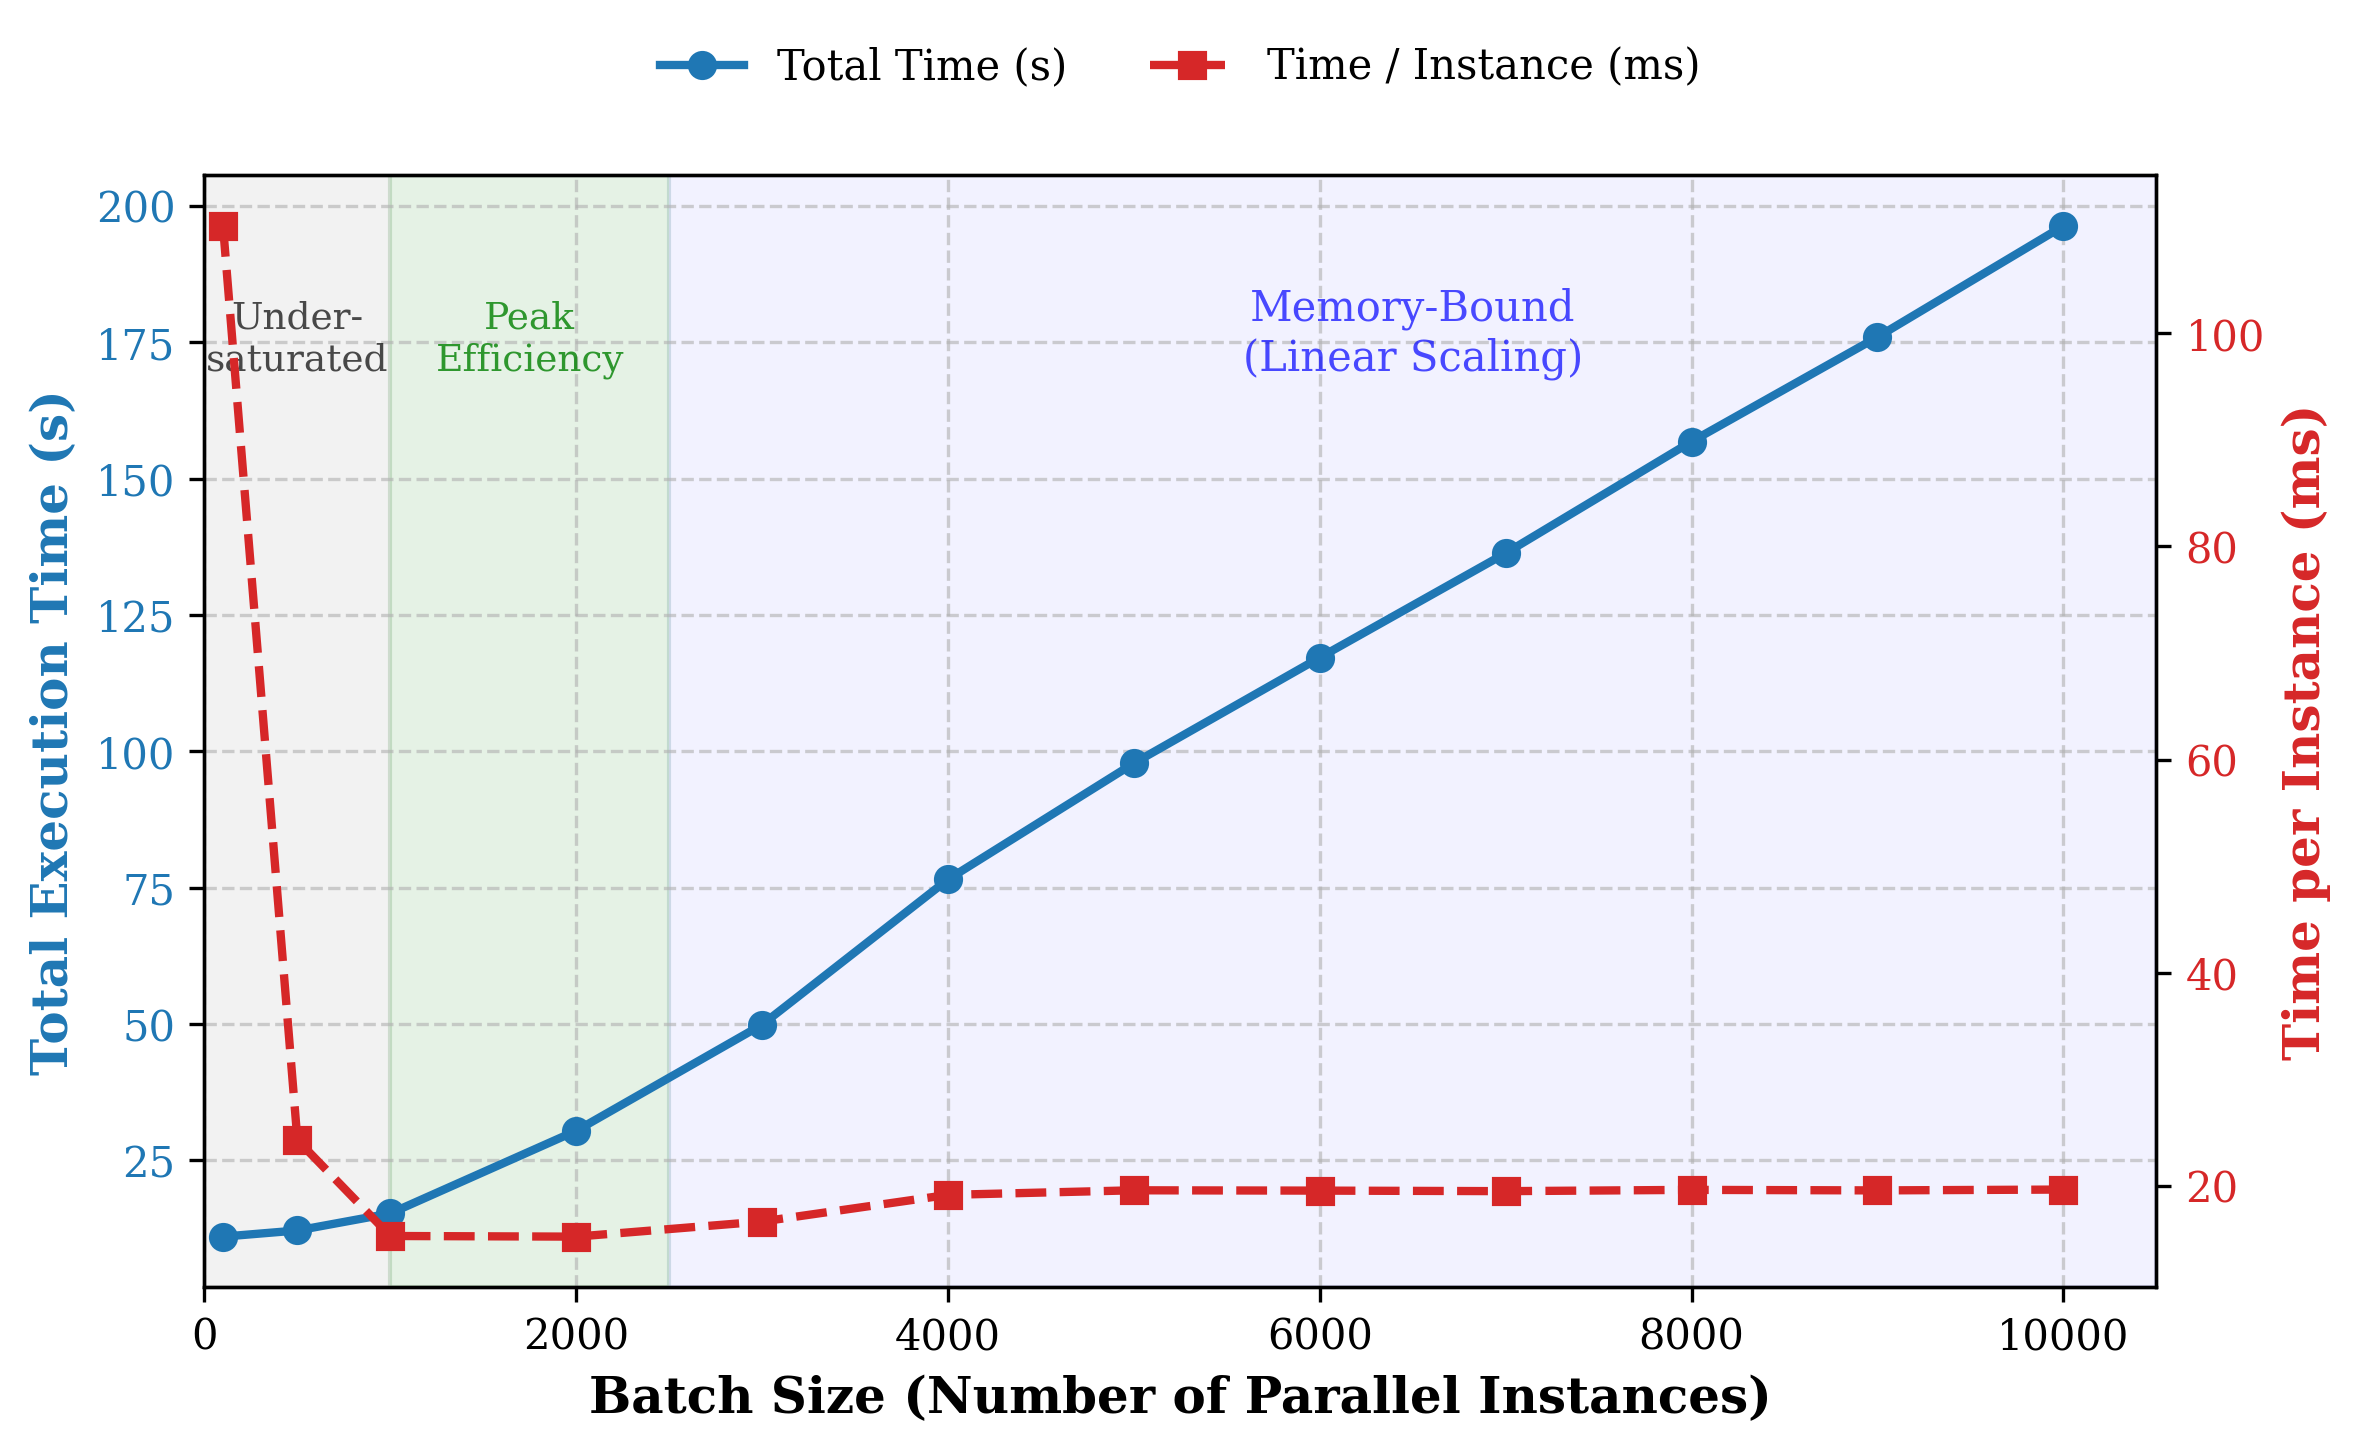
\includegraphics[width=\linewidth]{batch_scaling_analysis.png}
    \caption{GPU Batched Execution Scaling ($N=100$, $10{,}000$ steps). The dual-axis plot highlights the total execution time (blue, left axis) and the time per instance (red, right axis), revealing the under-saturated, peak efficiency, and memory-bound hardware regimes.}
    \label{fig:batch_scaling}
\end{figure}


\begin{table}[t]
\centering
\small
\caption{Impact of batch size on GPU execution time. \textbf{Setup:} $N=100$, $10{,}000$ steps.}
\label{tab:batch_scaling}
\begin{tabular}{r r c}
\toprule
\textbf{Batch Size} & \textbf{Time (s)} & \textbf{Time per Instance (ms)} \\
\midrule
100    & 11.01  & 110.09 \\
500    & 12.14  & 24.28 \\
1,000  & 15.27  & 15.27 \\
2,000  & 30.42  & 15.21 \\
3,000  & 49.88  & 16.63 \\
4,000  & 76.51  & 19.13 \\
5,000  & 97.82  & 19.56 \\
6,000  & 117.19 & 19.53 \\
7,000  & 136.33 & 19.48 \\
8,000  & 156.80 & 19.60 \\
9,000  & 175.96 & 19.55 \\
10,000 & 196.33 & 19.63 \\
\bottomrule
\end{tabular}
\end{table}

% ---------------------------------------------------------
% MAIN RESULTS / STATE OF THE ART
% ---------------------------------------------------------

\subsection{Comparison with State-of-the-Art}
We evaluate the performance of our LG-SA model against established classical and learning-based methods on $10{,}000$ instances generated following \citet{nazari_reinforcement_2018}.
Classical solvers include LKH3 \citep{helsgaun_extension_2017} and OR-Tools \citep{ortools_routing}. Learning-based methods comprise constructive approaches such as the Attention Model (AM) \citep{kool_attention_2019}, the RL baseline of \citet{nazari_reinforcement_2018}, and POMO \citep{kwon_pomo_2021}. We also compare against neural improvement heuristics: LIH \citep{wu_learning_2022}, CDCP \citep{garcia-torres_combining_2022}, DACT \citep{ma_learning_2021}, NLNS \citep{hottung_neural_2022}, and LCP \citep{kim_learning_2021}.

We report wall-clock times for the full test set. To ensure fairness, OR-Tools was initially re-evaluated with a per-instance time limit calculated by dividing LG-SA's total runtime at 100,000 steps by the 10,000 test instances. Additionally, to observe its performance under a more relaxed computational budget, we also ran OR-Tools with a time limit of 0.5 seconds per problem, which is more than twice the time required by LG-SA. As shown in Table \ref{tab:vs_baselines_combined}, our method achieves competitive results, particularly regarding the trade-off between solution quality and wall-clock time on large batches.

\begin{table}[t]
\centering
\small
\setlength{\tabcolsep}{5pt}
\caption{Comparison of LG-SA with established baselines. LG-SA uses the curriculum-trained model (best cost $16.343$ at $10$k steps on Nazari $N{=}100$). Runtime is for the full test set of 10{,}000 instances. \textbf{Bold}: best cost per column; \underline{underline}: best among learning methods.}
\label{tab:vs_baselines_combined}
\begin{tabular}{@{}l r r r r@{}}
\toprule
& \multicolumn{2}{c}{$N=50$} & \multicolumn{2}{c}{$N=100$} \\
\cmidrule(lr){2-3} \cmidrule(lr){4-5}
Method & Cost & Time & Cost & Time \\
\midrule
\multicolumn{5}{@{}l}{\textit{Classical Solvers}} \\[1pt]
\quad LKH3 & \textbf{10.38} & 5h 00m & \textbf{15.68} & 9h 00m \\
\quad OR-Tools (matched time) & 10.86 & 15m 33s & 16.58 & 31m 39s \\
\quad OR-Tools (0.5s) & 10.66 & 1h 23m & 16.43 & 1h 23m \\
\quad OR-Tools (1s) & 10.57 & 2h 46m & 16.32 & 2h 46m \\
\addlinespace[4pt]
\multicolumn{5}{@{}l}{\textit{Constructive Learning}} \\[1pt]
\quad AM (greedy) & 10.98 & 3s & 16.80 & 8s \\
\quad POMO & 10.74 & 1s & 16.15 & 3s \\
\quad POMO x 8 augment & 10.42 & 26s & 15.73 & 2m \\
\quad RL (Beam 10) & 11.15 & -- & 16.96 & -- \\
\addlinespace[4pt]
\multicolumn{5}{@{}l}{\textit{Neural Improvement}} \\[1pt]
\quad NLNS & 10.54 & 24m & 15.99 & 1h 02m \\
\quad LIH & 10.45 & 4h & 16.03 & 5h \\
\quad CDCP & 10.47 & 10h & 15.85 & 19h \\
\quad DACT ($T$=1k) & 10.55 & 16m & 16.20 & 41m \\
\quad DACT ($T$=5k) & 10.46 & 1h 30m & 15.95 & 3h 30m \\
\quad DACT ($T$=10k) x 6 augment & 10.38 & 16h & 15.74 & 41h \\
\quad LCP & 10.54 & 34m & 16.03 & 1h 15m \\
\addlinespace[4pt]
\multicolumn{5}{@{}l}{\textit{SA, no policy (ablation)}} \\[1pt]
\quad 10k steps & 16.14 & 14s & 32.37 & 25s \\
\quad 100k steps & 14.05 & 2m 21s & 26.71 & 4m 15s \\
\midrule
\multicolumn{5}{@{}l}{\textit{LG-SA (ours)}} \\[1pt]
\quad 10k steps & 10.67 & 1m 33s & 16.34 & 3m 13s \\
\quad 10k steps x 8 augment & 10.48 & 12m 24s & 16.05 & 26m \\
\quad 100k steps & 10.50 & 15m 33s & 15.98 & 31m 39s \\
\quad 200k steps & 10.47 & 31m 07s & 15.91 & 1h 03m \\
\quad 500k steps & 10.43 & 1h 12m & 15.85 & 2h 15m \\
\quad 1{,}000k steps & \underline{10.41} & 2h 25m & \underline{15.81} & 4h 30m \\
\bottomrule
\end{tabular}
\end{table}

\paragraph{Pareto-optimal regime.}
Table~\ref{tab:vs_baselines_combined} reveals that LG-SA occupies a distinct region of the cost--time Pareto frontier. At $10{,}000$ steps with $\times 8$ augmentation, LG-SA reaches $16.05$ on $N{=}100$ in $26$ minutes — outperforming all neural improvement methods at comparable or shorter runtime (NLNS $15.99$ in $1$h$02$m, DACT $T{=}5$k $15.95$ in $3$h$30$m, LIH $16.03$ in $5$h, LCP $16.03$ in $1$h$15$m), and matching OR-Tools at twice its budget ($16.32$ in $2$h$46$m). At extended budgets ($1{,}000$k steps), LG-SA reaches $15.81$, the best among learning-based methods that do not use augmentation, and within $0.13$ of LKH3 at half its wall-clock time.
 
\paragraph{Augmentation effectiveness.}
Following the instance-augmentation strategy introduced by \citet{kwon_pomo_2021} and adopted in subsequent neural improvement methods such as DACT \citep{ma_learning_2021}, the $\times 8$ instance augmentation provides a substantial gain at fixed step count: from $16.34 \to 16.05$ on $N{=}100$ ($-0.29$ absolute, $-1.8\%$ relative) and from $10.67 \to 10.48$ on $N{=}50$ ($-0.19$, $-1.8\%$). Notably, LG-SA at $10$k steps with augmentation ($16.05$, $26$m) outperforms LG-SA at $200$k steps without augmentation ($15.91$ on $N{=}100$ in $1$h$03$m only marginally better), indicating that diversification via augmentation is roughly as effective as a $20\times$ increase in step budget --- but at $2.4\times$ less wall-clock time. This confirms that the residual gap at large step counts is dominated by attractor diversity rather than insufficient local refinement. We note that the reported $\times 8$-augmented runtime ($26$m on $N{=}100$, $12$m$24$s on $N{=}50$) reflects sequential execution of the $8$ augmentations on our hardware: with $10{,}000$ instances already saturating GPU compute at $99\%$ utilization for a single augmentation, the $8\times$ memory expansion required for parallel execution exceeded our available GPU memory ($12$~GB). On hardware with sufficient memory ($\geq 28$~GB for $N{=}100$ at this batch size), the $8$ augmentations can be processed as a single $8B$-batch in essentially the same wall-clock time as a single augmentation, which would place augmented LG-SA strictly on the Pareto frontier.
 
\paragraph{Comparison with construction-based methods.}
POMO \citep{kwon_pomo_2021} with $\times 8$ augmentation achieves $15.73$ in $2$ minutes on $N{=}100$, outperforming our $10$k-step augmented variant. However, this comparison reflects a fundamental difference in computational regimes: POMO performs a single forward pass per trajectory, whereas LG-SA performs $10{,}000$ sequential improvement steps with full feature recomputation at each step. The two methods occupy different points on the speed-quality trade-off curve and should be viewed as complementary rather than directly competing --- LG-SA's strength lies in its ability to continue refining beyond construction-time quality, as evidenced by its monotonic improvement from $16.34$ at $10$k steps to $15.81$ at $1{,}000$k steps. A similar pattern is observed for DACT \citep{ma_learning_2021}, where the $\times 6$-augmented variant at $T{=}10$k achieves $15.74$ on $N{=}100$ but at the cost of $41$ hours of wall-clock time --- nearly two orders of magnitude slower than augmented LG-SA at $10$k steps for a comparable cost.
 
\paragraph{The role of the learned policy.}
The SA-only ablation (no policy) reaches only $26.71$ on $N{=}100$ at $100$k steps, compared to $15.98$ for LG-SA at the same step count --- a gap of $10.73$ absolute units, or $+67\%$ in relative cost. This isolates the contribution of the learned actor: under identical Metropolis acceptance and identical move types (insertion), the learned proposal distribution accounts for essentially all of the quality of the final solution. The temperature schedule alone is incapable of producing competitive solutions on this benchmark, confirming that LG-SA's performance is not attributable to SA itself but to the learned guidance.
% ---------------------------------------------------------
% GENERALIZATION ON CVRPLIB (UCHOA BENCHMARK)
% ---------------------------------------------------------

\subsection{Generalization on CVRPLIB (Uchoa Benchmark)}
\label{sec:uchoa_generalization}

To further assess the generalization capability of LG-SA, we evaluate it on a subset of Set~X from the CVRPLIB benchmark \citep{uchoa_new_2017}. Set~X contains 100 instances spanning sizes from 101 to 1001 customers; following \citet{ma_learning_2021}, we restrict our evaluation to the 22 smallest instances (sizes 101–200) to enable a direct comparison.

These instances are notably challenging for generalization: depot positions span random (R), central (C), and eccentric (E) placements, while customer distributions include random (R), clustered (C), and mixed random-cluster (RC) configurations — all far from the uniform distribution used during training.

We compare against the baselines reported by \citet{ma_learning_2021}: LIH \citep{wu_learning_2022}, OR-Tools \citep{ortools_routing}, AM-sampling ($N{=}10\text{k}$) \citep{kool_attention_2019}, POMO $\times$8 augment \citep{kwon_pomo_2021}, and DACT \citep{ma_learning_2021} in several configurations.
Gap values for all competing methods are taken directly from \citet{ma_learning_2021}; our results are computed against the same BKS values provided in the CVRPLIB repository.

\paragraph{Experimental setup.}
Since CVRPLIB instances have heterogeneous sizes, we cannot form uniform batches directly.
We handle this by padding each instance with \emph{ghost nodes} (zero-demand customers placed at the depot) up to the largest instance in the batch, allowing all instances to be processed in a single GPU forward pass.

Ghost nodes are masked throughout and never appear in any solution.
We repeat each run with 10 different random seeds and report the best and average gap over those runs.
Runtimes are measured on the full Set~X (100 instances): at 1\,M SA steps the total wall-clock time is approximately 25 minutes ($\approx$\,15\,s per instance); at 100\,k steps it is about 2.5 minutes ($\approx$\,1.5\,s per instance).


\paragraph{Results.}
Table~\ref{tab:uchoa_benchmark} reports optimality gaps relative to BKS for all methods.
Overall, LG-SA (1M, Best) achieves an average optimality gap of 4.21\% (3.01\% on [100,\,150), 5.41\% on [150,\,200]).
This outperforms DACT ($T$=5k, Best) at 4.32\%, the strongest prior result at comparable inference without augmentation.
The strongest published result, DACT with 6$\times$ augmentation, achieves 2.97\%/4.09\% by exploiting sixfold inference compute; LG-SA matches it on several individual instances without any augmentation.
Importantly, LG-SA is evaluated \emph{without any augmentation or problem-specific fine-tuning}, yet remains competitive across all neural improvement baselines.
The average-over-seeds result (LG-SA 1M Avg, 5.28\%) confirms stability across runs.

At 100k steps, LG-SA already matches or beats several strong baselines (OR-Tools, AM-sampling, LIH) at a fraction of the compute cost, demonstrating a favourable quality-time trade-off.
As expected, neural improvement methods (LIH, DACT, LG-SA) generalize considerably better than neural construction methods (AM-sampling, POMO), consistent with the observations in \citet{ma_learning_2021}.
Instance-level results for all 100 Set~X instances against classical metaheuristics (AILS-II, HGS-CVRP, LKH-3, OR-Tools) are reported in Appendix Table~\ref{tab:setx_full}.

\clearpage
\onecolumn
\begin{landscape}
\centering
\scriptsize
\setlength{\tabcolsep}{3pt}
\begin{longtable}{@{}l c c r rr rrrr rr rr rr rr@{}}
\caption{Optimality gaps (\%) on CVRPLIB Set~X \citep{uchoa_new_2017} relative to BKS. Results for LIH, DACT, OR-Tools, AM, and POMO are taken from \citet{ma_learning_2021}. LG-SA: 10 seeds, Best/Avg reported. D.: Depot type; N.: Node type; OR-T.: OR-Tools; AM: AM-sampling ($N$=10k); POMO: POMO$\times$8; LIH-M: LIH ($T$=5k, $M$=100).}
\label{tab:uchoa_benchmark} \\
\toprule
& & & & \multicolumn{2}{c}{DACT ($T$=5k)} & \multicolumn{4}{c}{Baselines} & \multicolumn{2}{c}{DACT ($T$=10k)} & \multicolumn{2}{c}{DACT ($\times$6 aug.)} & \multicolumn{2}{c}{LG-SA (100k)} & \multicolumn{2}{c}{LG-SA (1M)} \\
\cmidrule(lr){5-6}\cmidrule(lr){7-10}\cmidrule(lr){11-12}\cmidrule(lr){13-14}\cmidrule(lr){15-16}\cmidrule(lr){17-18}
Instance & D. & N. & LIH & Best & Avg & OR-T. & AM & POMO & LIH-M & Best & Avg & Best & Avg & Best & Avg & Best & Avg \\
\midrule
\endfirsthead
\toprule
& & & & \multicolumn{2}{c}{DACT ($T$=5k)} & \multicolumn{4}{c}{Baselines} & \multicolumn{2}{c}{DACT ($T$=10k)} & \multicolumn{2}{c}{DACT ($\times$6 aug.)} & \multicolumn{2}{c}{LG-SA (100k)} & \multicolumn{2}{c}{LG-SA (1M)} \\
\cmidrule(lr){5-6}\cmidrule(lr){7-10}\cmidrule(lr){11-12}\cmidrule(lr){13-14}\cmidrule(lr){15-16}\cmidrule(lr){17-18}
Instance & D. & N. & LIH & Best & Avg & OR-T. & AM & POMO & LIH-M & Best & Avg & Best & Avg & Best & Avg & Best & Avg \\
\midrule
\endhead
\midrule
\multicolumn{18}{r}{Continued on next page} \\
\midrule
\endfoot
\bottomrule
\endlastfoot
X-n101-k25 & R & R & 7.70\% & 1.86\% & 3.49\% & 6.57\% & 32.95\% & 3.64\% & 5.60\% & 1.68\% & 3.11\% & 1.32\% & 1.86\% & 3.40\% & 4.78\% & 2.45\% & 3.43\% \\
X-n106-k14 & E & C & 4.86\% & 2.33\% & 3.00\% & 3.72\% & 6.78\% & 1.85\% & 2.83\% & 2.28\% & 2.77\% & 1.72\% & 2.09\% & 4.30\% & 5.00\% & 2.56\% & 3.61\% \\
X-n110-k13 & C & R & 6.39\% & 0.41\% & 2.64\% & 7.87\% & 3.15\% & 2.05\% & 4.40\% & 0.37\% & 2.38\% & 0.00\% & 1.10\% & 3.17\% & 4.09\% & 1.30\% & 2.03\% \\
X-n115-k10 & C & R & 13.32\% & 1.23\% & 1.80\% & 4.50\% & 7.52\% & 3.49\% & 5.19\% & 0.08\% & 1.43\% & 0.02\% & 0.68\% & 3.05\% & 4.58\% & 2.68\% & 3.21\% \\
X-n120-k6 & E & RC & 16.16\% & 3.52\% & 6.32\% & 6.83\% & 4.54\% & 2.12\% & 5.56\% & 3.49\% & 6.01\% & 2.71\% & 4.00\% & 1.91\% & 3.47\% & 1.78\% & 2.29\% \\
X-n125-k30 & R & C & 8.79\% & 5.50\% & 6.71\% & 5.63\% & 35.16\% & 7.14\% & 4.71\% & 4.76\% & 6.01\% & 4.76\% & 5.51\% & 5.72\% & 6.37\% & 4.32\% & 5.38\% \\
X-n129-k18 & E & RC & 11.01\% & 4.06\% & 5.72\% & 8.37\% & 4.00\% & 0.97\% & 4.63\% & 3.98\% & 5.28\% & 3.48\% & 3.91\% & 4.49\% & 6.06\% & 3.09\% & 4.49\% \\
X-n134-k13 & R & C & 16.06\% & 4.85\% & 7.17\% & 21.61\% & 20.13\% & 4.22\% & 8.88\% & 3.77\% & 6.40\% & 2.32\% & 3.28\% & 8.47\% & 9.93\% & 7.02\% & 8.22\% \\
X-n139-k10 & C & R & 14.99\% & 1.82\% & 3.47\% & 12.02\% & 4.30\% & 2.28\% & 4.90\% & 1.65\% & 3.05\% & 0.53\% & 1.13\% & 3.38\% & 5.56\% & 1.72\% & 3.47\% \\
X-n143-k7 & E & R & 20.20\% & 4.59\% & 5.86\% & 11.27\% & 8.88\% & 2.79\% & 6.61\% & 3.92\% & 5.15\% & 0.89\% & 3.37\% & 3.20\% & 5.42\% & 2.79\% & 3.97\% \\
X-n148-k46 & R & RC & 16.38\% & 4.09\% & 5.21\% & 7.80\% & 79.53\% & 19.88\% & 3.60\% & 3.61\% & 4.75\% & 2.60\% & 4.24\% & 4.26\% & 5.26\% & 3.40\% & 4.33\% \\
X-n153-k22 & C & C & 22.94\% & 6.10\% & 8.98\% & 8.01\% & 78.11\% & 12.16\% & 4.53\% & 4.63\% & 7.62\% & 3.22\% & 4.26\% & 10.99\% & 14.54\% & 9.24\% & 11.24\% \\
X-n157-k13 & R & C & 17.15\% & 3.24\% & 3.78\% & 2.57\% & 16.30\% & 2.79\% & 3.60\% & 2.70\% & 3.36\% & 2.09\% & 2.60\% & 8.31\% & 9.69\% & 6.04\% & 7.28\% \\
X-n162-k11 & C & RC & 19.16\% & 2.53\% & 3.98\% & 6.31\% & 6.37\% & 4.77\% & 5.26\% & 1.82\% & 2.68\% & 1.10\% & 1.57\% & 5.30\% & 7.15\% & 3.49\% & 4.20\% \\
X-n167-k10 & E & R & 18.52\% & 5.03\% & 6.36\% & 9.34\% & 8.41\% & 4.05\% & 8.27\% & 4.36\% & 5.75\% & 4.05\% & 4.83\% & 3.53\% & 5.10\% & 2.40\% & 3.07\% \\
X-n172-k51 & C & RC & 12.06\% & 4.44\% & 6.50\% & 10.74\% & 85.37\% & 21.99\% & 4.36\% & 3.66\% & 5.42\% & 3.37\% & 3.78\% & 5.56\% & 6.33\% & 4.55\% & 5.59\% \\
X-n176-k26 & E & R & 19.49\% & 8.53\% & 13.23\% & 8.99\% & 20.39\% & 10.27\% & 6.16\% & 7.74\% & 10.91\% & 7.74\% & 9.13\% & 8.25\% & 10.17\% & 5.89\% & 7.66\% \\
X-n181-k23 & R & C & 6.27\% & 3.27\% & 3.84\% & 2.94\% & 6.45\% & 2.08\% & 2.08\% & 3.05\% & 3.65\% & 1.89\% & 2.51\% & 5.86\% & 6.57\% & 4.50\% & 5.25\% \\
X-n186-k15 & R & R & 17.71\% & 7.40\% & 9.15\% & 7.75\% & 6.01\% & 2.15\% & 7.65\% & 6.80\% & 8.01\% & 5.01\% & 6.10\% & 5.36\% & 6.77\% & 2.66\% & 4.28\% \\
X-n190-k8 & E & C & 18.64\% & 7.00\% & 8.69\% & 6.53\% & 46.61\% & 9.25\% & 6.78\% & 6.36\% & 7.86\% & 5.81\% & 6.42\% & 12.04\% & 13.85\% & 10.92\% & 11.71\% \\
X-n195-k51 & C & RC & 17.04\% & 6.78\% & 8.39\% & 13.76\% & 79.26\% & 9.23\% & 4.47\% & 6.60\% & 7.74\% & 5.14\% & 6.25\% & 5.99\% & 7.24\% & 3.98\% & 5.00\% \\
X-n200-k36 & R & C & 9.60\% & 6.43\% & 7.26\% & 4.15\% & 26.25\% & 5.01\% & 4.26\% & 6.30\% & 7.08\% & 5.54\% & 6.07\% & 6.49\% & 7.59\% & 5.85\% & 6.48\% \\
\midrule
\textbf{Avg.\ [100,150)} & -- & -- & \textbf{12.35\%} & \textbf{3.11\%} & \textbf{4.67\%} & \textbf{8.74\%} & \textbf{18.81\%} & \textbf{4.58\%} & \textbf{5.17\%} & \textbf{2.69\%} & \textbf{4.21\%} & \textbf{1.85\%} & \textbf{2.83\%} & \textbf{4.12\%} & \textbf{5.50\%} & \textbf{3.01\%} & \textbf{4.04\%} \\
\textbf{Avg.\ [150,200]} & -- & -- & \textbf{16.24\%} & \textbf{5.52\%} & \textbf{7.29\%} & \textbf{7.37\%} & \textbf{34.50\%} & \textbf{7.61\%} & \textbf{5.22\%} & \textbf{4.91\%} & \textbf{6.37\%} & \textbf{4.09\%} & \textbf{4.87\%} & \textbf{7.06\%} & \textbf{8.64\%} & \textbf{5.41\%} & \textbf{6.52\%} \\
\textbf{Avg.\ all} & -- & -- & \textbf{14.29\%} & \textbf{4.32\%} & \textbf{5.98\%} & \textbf{8.06\%} & \textbf{26.66\%} & \textbf{6.10\%} & \textbf{5.20\%} & \textbf{3.80\%} & \textbf{5.29\%} & \textbf{2.97\%} & \textbf{3.85\%} & \textbf{5.59\%} & \textbf{7.07\%} & \textbf{4.21\%} & \textbf{5.28\%} \\
\end{longtable}
\end{landscape}
\twocolumn

% -------------------------------------------------------
\subsection{Generalization on Set XML (10,000-instance Benchmark)}
\label{sec:xml_generalization}

To evaluate LG-SA at scale on a structurally diverse benchmark, we test on the 10,000-instance dataset from \citet{queiroga_10000_nodate} (Set XML). The dataset follows the same generation scheme as \citet{uchoa_new_2017}, producing 2D Euclidean instances with systematic variation across four structural dimensions:
\begin{itemize}
    \item \textbf{Depot positioning:} Random (R), Centered (C), Cornered (E).
    \item \textbf{Customer positioning:} Random (R), Clustered (C), Random-Clustered (RC).
    \item \textbf{Demand distribution:} Unitary (U), small values with large CV (1--10), small values with small CV (5--10), large values with large CV (1--100), large values with small CV (50--100), quadrant-dependent (Q), many small and few large values (SL).
    \item \textbf{Average route size $r$:} Very short (VS) ($r \in [3,5]$), Short (S) ($[5,8]$), Medium (M) ($[8,12]$), Long (L) ($[12,16]$), Very long (VL) ($[16,25]$), Ultra long (UL) ($[25,50]$).
\end{itemize}

\paragraph{Experimental setup.}
LG-SA is evaluated with $100{,}000$ SA steps per instance, repeated over 10 independent seeds; Best and Mean optimality gaps are reported. The full 10,000-instance dataset is processed as a single batched GPU run, completing in approximately 31 minutes in total ($\approx$\,$0.19$\,s per instance). Classical baselines (AILS-II, HGS-CVRP, LKH-3, OR-Tools) are taken from \citet{queiroga_10000_nodate}, where each method was run with 10 independent runs per instance under a one-minute CPU time limit.

\paragraph{Results.}
Table~\ref{tab:xml_by_groups} reports the average optimality gap (\%) for each subgroup. Overall, LG-SA (100k) achieves gaps of 3.62\% (Best) and 5.25\% (Mean), versus 1.01\%/1.45\% for OR-Tools. As expected, dedicated metaheuristics (AILS-II, HGS-CVRP) operate near-optimally at gaps below 0.01\%, while LKH-3 reaches 0.25\%/0.48\% overall.

Across subgroups, LG-SA performs best on randomly distributed customers (R: 2.54\% Best) and on medium-to-long routes (M/L: $\approx$\,3.0\% Best), configurations closer to the training distribution. The hardest cases are clustered customers (C: 4.93\% Best) and ultra-long routes (UL: 4.85\% / 7.32\%). This contrasts with classical methods, which benefit from simpler problem structure as route length increases: LKH-3's gap drops from 0.88\% on very-short routes to 0.004\% on ultra-long routes, and OR-Tools from 1.09\% to 0.27\%. LG-SA exhibits the opposite trend on ultra-long routes, likely because instances with very few, very long routes fall outside its training distribution and provide fewer independent improvement opportunities for the local insertion operator. Demand distribution has comparatively little effect on LG-SA's relative standing, with gaps ranging from 3.32\% (Unitary) to 4.00\% (SL).

The key comparison is computational: LG-SA processes the entire 10,000-instance benchmark in 31 minutes on a single GPU, achieving roughly $\approx$\,$0.19$\,s per instance. This is over 300 times faster per instance than the one-minute baseline budget, at a cost of approximately 3.6$\times$ the optimality gap relative to OR-Tools. LG-SA thus occupies a distinct operational regime suited for high-throughput scenarios where thousands of instances must be solved in parallel.

\begin{table*}[t]
\centering
\caption{Average optimality gap (\%) on the 10,000-instance Set XML benchmark \citep{queiroga_10000_nodate}, grouped by structural attribute. Classical baselines: 10 independent runs per instance, 1-minute CPU time limit. LG-SA (100k): 10 seeds, $100{,}000$ SA steps, full batch on GPU ($\approx$\,$0.19$\,s per instance). Entries report Best and Mean gap over runs.}
\label{tab:xml_by_groups}
\small
\begin{tabular}{llrrrrrrrrrr}
\toprule
Attribute & Level & \multicolumn{2}{c}{AILS-II} & \multicolumn{2}{c}{HGS-CVRP} & \multicolumn{2}{c}{LKH-3} & \multicolumn{2}{c}{OR-Tools} & \multicolumn{2}{c}{LG-SA (100k)} \\
 &  & Best & Mean & Best & Mean & Best & Mean & Best & Mean & Best & Mean \\
\midrule
Depot pos. & R & 0.002 & 0.008 & 0.001 & 0.002 & 0.273 & 0.506 & 1.047 & 1.496 & 3.630 & 5.280 \\
Depot pos. & C & 0.004 & 0.009 & 0.001 & 0.001 & 0.323 & 0.550 & 0.695 & 1.099 & 3.390 & 5.060 \\
Depot pos. & E & 0.002 & 0.010 & 0.003 & 0.006 & 0.151 & 0.379 & 1.280 & 1.766 & 3.840 & 5.430 \\
Customer pos. & R & 0.003 & 0.011 & 0.000 & 0.002 & 0.298 & 0.577 & 1.150 & 1.557 & 2.540 & 4.110 \\
Customer pos. & C & 0.002 & 0.007 & 0.003 & 0.006 & 0.183 & 0.345 & 0.840 & 1.301 & 4.930 & 6.570 \\
Customer pos. & RC & 0.002 & 0.010 & 0.001 & 0.002 & 0.268 & 0.514 & 1.028 & 1.498 & 3.410 & 5.100 \\
Demand dist. & U & 0.000 & 0.001 & 0.000 & 0.000 & 0.010 & 0.089 & 0.632 & 0.940 & 3.320 & 4.730 \\
Demand dist. & 1--10 & 0.001 & 0.008 & 0.001 & 0.003 & 0.085 & 0.285 & 1.162 & 1.617 & 3.530 & 5.100 \\
Demand dist. & 5--10 & 0.001 & 0.006 & 0.000 & 0.001 & 0.103 & 0.304 & 1.108 & 1.550 & 3.520 & 5.090 \\
Demand dist. & 1--100 & 0.003 & 0.014 & 0.003 & 0.006 & 0.325 & 0.648 & 1.185 & 1.672 & 3.600 & 5.180 \\
Demand dist. & 50--100 & 0.005 & 0.014 & 0.000 & 0.002 & 0.345 & 0.650 & 1.152 & 1.596 & 3.680 & 5.280 \\
Demand dist. & Q & 0.003 & 0.012 & 0.001 & 0.004 & 0.484 & 0.804 & 1.141 & 1.632 & 3.680 & 5.400 \\
Demand dist. & SL & 0.004 & 0.010 & 0.005 & 0.008 & 0.441 & 0.602 & 0.666 & 1.162 & 4.000 & 5.990 \\
Route size $r$ & VS & 0.008 & 0.019 & 0.004 & 0.006 & 0.880 & 1.288 & 1.206 & 1.641 & 3.830 & 5.240 \\
Route size $r$ & S & 0.003 & 0.014 & 0.001 & 0.004 & 0.454 & 0.802 & 1.415 & 1.963 & 3.500 & 4.920 \\
Route size $r$ & M & 0.001 & 0.008 & 0.002 & 0.004 & 0.156 & 0.433 & 1.315 & 1.839 & 3.040 & 4.410 \\
Route size $r$ & L & 0.001 & 0.007 & 0.001 & 0.002 & 0.079 & 0.290 & 1.087 & 1.572 & 2.980 & 4.380 \\
Route size $r$ & VL & 0.001 & 0.005 & 0.001 & 0.002 & 0.025 & 0.159 & 0.749 & 1.158 & 3.530 & 5.260 \\
Route size $r$ & UL & 0.001 & 0.002 & 0.001 & 0.002 & 0.004 & 0.033 & 0.266 & 0.541 & 4.850 & 7.320 \\
\midrule
\textbf{Overall} &  & \textbf{0.002} & \textbf{0.009} & \textbf{0.001} & \textbf{0.003} & \textbf{0.250} & \textbf{0.479} & \textbf{1.006} & \textbf{1.452} & \textbf{3.620} & \textbf{5.250} \\
\bottomrule
\end{tabular}

\end{table*}

\section{Conclusion}
\label{sec:conclusion}

We presented LG-SA, a hybrid framework that combines classical Simulated Annealing with a PPO-trained lightweight neural policy for the Capacitated Vehicle Routing Problem. The policy learns to propose promising node-insertion moves from a rich, dynamic feature representation, guided by the Metropolis acceptance criterion and trained with a shallow sigmoid curriculum that avoids catastrophic forgetting.

Our comprehensive empirical study yields several non-obvious findings. \textbf{First}, the interaction between operator and feasibility strategy is critical: insertion with proactive action masking substantially outperforms all other combinations, whereas swap and two-opt benefit from reactive constraint handling. \textbf{Second}, local geometric features --- specifically the detour cost and immediate neighbor coordinates --- are the primary drivers of solution quality; spatial density metrics ($\rho^{(5)}, \rho^{(10\%)}, \rho^{(33\%)}$) are largely redundant and can be pruned without performance loss. \textbf{Third}, the optimal curriculum depth for a lightweight improvement policy is far shallower ($\xi_{\text{CL}} \approx 120$ pre-steps) than for heavyweight constructive policies; exceeding this threshold induces catastrophic forgetting. \textbf{Fourth}, random initialization acts as a powerful regularizer: a model trained exclusively on random starting solutions generalizes more robustly than any specialist-trained model across all initialization types and even across unseen instance distributions. \textbf{Fifth}, dense, step-level immediate rewards substantially outperform sparse or terminal reward formulations, confirming that fine-grained feedback is essential for learning effective local search policies with PPO.

LG-SA achieves a routing cost of $15.81$ at $1$M steps on the Nazari $N=100$ benchmark, a $4.21\%$ average optimality gap on CVRPLIB Set~X without augmentation, and processes $10{,}000$ structurally diverse instances in 31 minutes on a single GPU. The method scales near-linearly to graphs of $N=10{,}000$ nodes, with wall-clock times under 32 seconds at $10{,}000$ steps, making it well-suited for high-throughput industrial routing scenarios.

\paragraph{Limitations and Future Work.}
The primary limitation of LG-SA is its degradation on large instances: optimality gaps exceed $10\%$ on Set~X instances with $n>330$ nodes, where pointwise insertion becomes less effective and the problem structure drifts far from the training distribution. Incorporating large-neighborhood operators --- such as ALNS-style destroy-and-repair moves --- or population-based restarts may alleviate this. Additionally, the framework is currently constrained to a single fixed operator per run; a multi-operator strategy that dynamically selects among insertion, swap, and 2-opt could improve robustness across diverse instance types. Finally, extending LG-SA to richer VRP variants (time windows, heterogeneous fleets, multi-depot) and investigating learned or adaptive temperature schedules are natural directions for future work.

\newpage
\bibliography{bib}


\newpage
\section{Appendix}

\subsection{Full Set~X Results Against Classical Metaheuristics}
\label{app:setx_full}

Table~\ref{tab:setx_full} reports instance-level costs for all 100 Set~X instances \citep{uchoa_new_2017}, comparing LG-SA at 1M steps against the following classical baselines:
\begin{itemize}
    \item \textbf{HGS-CVRP} \citep{vidal_hybrid_2022}: A state-of-the-art hybrid genetic algorithm incorporating the SWAP* neighborhood.
    \item \textbf{AILS-II} \citep{maximo_adaptive_2021}: An adaptive iterated local search framework.
    \item \textbf{LKH-3} \citep{helsgaun_extension_2017}: An extension of the classic Lin-Kernighan-Helsgaun TSP solver adapted for the CVRP.
    \item \textbf{OR-Tools} \citep{ortools_routing}: A widely used commercial-grade routing library configured with Guided Local Search (GLS).
\end{itemize}

It is essential to contextualise the computational budgets before interpreting these results.
The classical baselines each perform \textbf{50 independent runs per instance with a 10-minute CPU time limit}, amounting to up to \textbf{500 CPU-minutes of compute per instance}.
LG-SA, by contrast, runs as a \textbf{single GPU-batched pass over all 100 instances simultaneously}, completing 1\,M SA steps in approximately 25 minutes total — around \textbf{15 seconds per instance}.
This represents a roughly \textbf{2{,}000$\times$ reduction in compute time}.

Under this asymmetry, LG-SA achieves an average optimality gap of 9.77\% (Best) across all instances, narrowing to 6.14\% for instances with $n < 330$ nodes.
The degradation on larger instances ($n > 330$, gap 13.26\%) reflects the inherent limitation of point-wise local search on large graphs, as discussed in Section~\ref{sec:uchoa_generalization}.
These results are not intended as a competitive claim against classical metaheuristics, but rather as an honest account of LG-SA's quality--speed frontier on real-world instances of varying scale.

\clearpage
\onecolumn
%\begin{landscape}
\centering
\scriptsize
\setlength{\tabcolsep}{3pt}
\begin{longtable}{@{}l rr rr rr rr rr@{}}
\caption{Full instance-level results on all 100 Set~X instances \citep{uchoa_new_2017}. Classical baselines: 50 independent runs, 10-minute CPU limit per run (up to 500 CPU-min per instance). LG-SA (1M): single GPU-batched run, $\approx$15\,s per instance. Costs are absolute tour lengths; gaps (\%) in summary rows are relative to BKS.}
\label{tab:setx_full} \\
\toprule
& \multicolumn{2}{c}{AILS-II} & \multicolumn{2}{c}{HGS-CVRP} & \multicolumn{2}{c}{LKH-3} & \multicolumn{2}{c}{OR-Tools} & \multicolumn{2}{c}{LG-SA (1M)} \\
\cmidrule(lr){2-3}\cmidrule(lr){4-5}\cmidrule(lr){6-7}\cmidrule(lr){8-9}\cmidrule(lr){10-11}
Instance & Best & Mean & Best & Mean & Best & Mean & Best & Mean & Best & Mean \\
\midrule
\endfirsthead
\toprule
& \multicolumn{2}{c}{AILS-II} & \multicolumn{2}{c}{HGS-CVRP} & \multicolumn{2}{c}{LKH-3} & \multicolumn{2}{c}{OR-Tools} & \multicolumn{2}{c}{LG-SA (1M)} \\
\cmidrule(lr){2-3}\cmidrule(lr){4-5}\cmidrule(lr){6-7}\cmidrule(lr){8-9}\cmidrule(lr){10-11}
Instance & Best & Mean & Best & Mean & Best & Mean & Best & Mean & Best & Mean \\
\midrule
\endhead
\midrule
\multicolumn{11}{r}{\textit{Continued on next page}} \\
\midrule
\endfoot
\bottomrule
\endlastfoot
X-n101-k25 & 27591.00 & 27591.00 & 27591.00 & 27591.00 & 29473.00 & 30679.70 & 27732.00 & 27971.50 & 28266.00 & 28536.40 \\
X-n106-k14 & 26362.00 & 26362.00 & 26362.00 & 26373.80 & 26362.00 & 26391.50 & 26672.00 & 26796.20 & 27037.00 & 27314.90 \\
X-n110-k13 & 14971.00 & 14971.00 & 14971.00 & 14971.00 & 14971.00 & 15006.50 & 14972.00 & 15078.10 & 15166.00 & 15274.60 \\
X-n115-k10 & 12747.00 & 12747.00 & 12747.00 & 12747.00 & 12747.00 & 12747.40 & 12757.00 & 12838.30 & 13089.00 & 13156.50 \\
X-n120-k6 & 13332.00 & 13332.00 & 13332.00 & 13332.00 & 13332.00 & 13335.20 & 13429.00 & 13527.70 & 13569.00 & 13637.10 \\
X-n125-k30 & 55539.00 & 55539.00 & 55539.00 & 55539.00 & 55546.00 & 55741.10 & 56361.00 & 56742.70 & 57938.00 & 58527.20 \\
X-n129-k18 & 28940.00 & 28940.40 & 28940.00 & 28940.00 & 28940.00 & 29022.70 & 29620.00 & 29703.40 & 29834.00 & 30239.60 \\
X-n134-k13 & 10916.00 & 10916.00 & 10916.00 & 10916.00 & 10916.00 & 10972.80 & 11046.00 & 11150.20 & 11682.00 & 11813.50 \\
X-n139-k10 & 13590.00 & 13590.00 & 13590.00 & 13590.00 & 13590.00 & 13616.40 & 13606.00 & 13675.60 & 13824.00 & 14061.10 \\
X-n143-k7 & 15700.00 & 15703.20 & 15700.00 & 15700.00 & 15700.00 & 15755.50 & 15928.00 & 16051.10 & 16138.00 & 16323.50 \\
X-n148-k46 & 43448.00 & 43448.00 & 43448.00 & 43448.00 & 43499.00 & 43597.70 & 43874.00 & 44199.00 & 44924.00 & 45330.20 \\
X-n153-k22 & 21220.00 & 21224.50 & 21223.00 & 21224.90 & 21418.00 & 21490.50 & 21488.00 & 21615.80 & 23181.00 & 23605.00 \\
X-n157-k13 & 16876.00 & 16876.00 & 16876.00 & 16876.00 & 16876.00 & 16879.90 & 16982.00 & 17057.30 & 17895.00 & 18104.10 \\
X-n162-k11 & 14138.00 & 14138.00 & 14138.00 & 14138.00 & 14138.00 & 14161.40 & 14214.00 & 14257.00 & 14631.00 & 14732.50 \\
X-n167-k10 & 20557.00 & 20557.30 & 20557.00 & 20557.00 & 20557.00 & 20603.30 & 21165.00 & 21268.90 & 21050.00 & 21187.50 \\
X-n172-k51 & 45607.00 & 45607.80 & 45607.00 & 45607.00 & 46580.00 & 46952.90 & 46350.00 & 46538.70 & 47684.00 & 48158.70 \\
X-n176-k26 & 47812.00 & 47812.00 & 47812.00 & 47812.00 & 47816.00 & 48037.30 & 49056.00 & 49250.80 & 50629.00 & 51473.20 \\
X-n181-k23 & 25569.00 & 25570.50 & 25569.00 & 25569.00 & 25571.00 & 25603.50 & 25770.00 & 25885.30 & 26720.00 & 26912.40 \\
X-n186-k15 & 24145.00 & 24149.40 & 24145.00 & 24145.00 & 24149.00 & 24307.10 & 24868.00 & 25023.00 & 24788.00 & 25178.90 \\
X-n190-k8 & 16980.00 & 16980.60 & 16980.00 & 16984.10 & 16992.00 & 17035.80 & 17342.00 & 17412.80 & 18835.00 & 18967.70 \\
X-n195-k51 & 44225.00 & 44256.50 & 44225.00 & 44225.00 & 46609.00 & 47560.50 & 45039.00 & 45370.60 & 45983.00 & 46435.80 \\
X-n200-k36 & 58578.00 & 58587.80 & 58578.00 & 58578.00 & 58657.00 & 58909.80 & 59745.00 & 60338.80 & 62005.00 & 62374.40 \\
X-n204-k19 & 19565.00 & 19565.70 & 19565.00 & 19565.00 & 19579.00 & 19723.40 & 19960.00 & 20172.70 & 20625.00 & 20818.10 \\
X-n209-k16 & 30656.00 & 30663.20 & 30656.00 & 30656.00 & 30679.00 & 30862.30 & 31681.00 & 31874.70 & 31608.00 & 31941.80 \\
X-n214-k11 & 10859.00 & 10869.10 & 10856.00 & 10859.30 & 10926.00 & 11094.00 & 11177.00 & 11310.70 & 12030.00 & 12203.10 \\
X-n219-k73 & 117595.00 & 117595.00 & 117595.00 & 117595.20 & 117613.00 & 117692.10 & 117854.00 & 117974.30 & 125748.00 & 126382.20 \\
X-n223-k34 & 40437.00 & 40446.30 & 40437.00 & 40437.20 & 40528.00 & 40713.90 & 41515.00 & 41886.50 & 42593.00 & 42932.50 \\
X-n228-k23 & 25742.00 & 25750.60 & 25742.00 & 25742.50 & 25757.00 & 25837.50 & 26279.00 & 26510.30 & 28455.00 & 28748.60 \\
X-n233-k16 & 19230.00 & 19256.20 & 19230.00 & 19230.00 & 19874.00 & 20218.20 & 19696.00 & 19895.70 & 20583.00 & 20773.40 \\
X-n237-k14 & 27042.00 & 27048.50 & 27042.00 & 27042.00 & 27051.00 & 27162.60 & 27583.00 & 27867.00 & 28087.00 & 28521.80 \\
X-n242-k48 & 82751.00 & 82808.70 & 82751.00 & 82801.30 & 82979.00 & 83291.50 & 85095.00 & 85515.70 & 88673.00 & 89823.20 \\
X-n247-k50 & 37274.00 & 37274.10 & 37274.00 & 37279.80 & 37409.00 & 37528.10 & 37819.00 & 38212.90 & 40079.00 & 40544.50 \\
X-n251-k28 & 38684.00 & 38722.10 & 38684.00 & 38688.10 & 38842.00 & 38970.50 & 39704.00 & 39998.70 & 40794.00 & 41352.40 \\
X-n256-k16 & 18839.00 & 18871.80 & 18839.00 & 18839.90 & 18931.00 & 19070.70 & 19034.00 & 19223.90 & 20636.00 & 20845.20 \\
X-n261-k13 & 26558.00 & 26574.40 & 26558.00 & 26561.40 & 26691.00 & 26879.50 & 27518.00 & 27850.60 & 28242.00 & 28437.50 \\
X-n266-k58 & 75478.00 & 75540.90 & 75478.00 & 75597.50 & 75792.00 & 76077.80 & 77410.00 & 77871.40 & 82578.00 & 83176.10 \\
X-n270-k35 & 35303.00 & 35329.40 & 35291.00 & 35302.40 & 36081.00 & 36628.60 & 36208.00 & 36600.60 & 37517.00 & 37939.50 \\
X-n275-k28 & 21245.00 & 21247.50 & 21245.00 & 21245.00 & 21245.00 & 21304.90 & 21858.00 & 22035.60 & 23536.00 & 23776.80 \\
X-n280-k17 & 33505.00 & 33563.40 & 33503.00 & 33545.00 & 33692.00 & 34042.80 & 34302.00 & 34949.70 & 35299.00 & 35793.00 \\
X-n284-k15 & 20215.00 & 20261.70 & 20216.00 & 20242.40 & 20350.00 & 20506.40 & 20815.00 & 21074.80 & 22893.00 & 23291.90 \\
X-n289-k60 & 95151.00 & 95263.00 & 95196.00 & 95284.80 & 97591.00 & 99190.40 & 97784.00 & 98266.90 & 103622.00 & 104961.90 \\
X-n294-k50 & 47169.00 & 47209.60 & 47161.00 & 47188.00 & 47515.00 & 47996.50 & 48651.00 & 49243.00 & 49950.00 & 50507.00 \\
X-n298-k31 & 34231.00 & 34259.80 & 34231.00 & 34233.60 & 34234.00 & 34633.30 & 35835.00 & 36513.70 & 36393.00 & 36726.00 \\
X-n303-k21 & 21736.00 & 21762.30 & 21738.00 & 21746.10 & 21852.00 & 21945.40 & 22164.00 & 22492.20 & 24348.00 & 24543.70 \\
X-n308-k13 & 25859.00 & 25878.90 & 25861.00 & 25872.60 & 26017.00 & 26217.40 & 26648.00 & 27111.00 & 28044.00 & 28473.50 \\
X-n313-k71 & 94044.00 & 94094.20 & 94044.00 & 94103.50 & 95640.00 & 96831.80 & 96377.00 & 96965.10 & 101305.00 & 102581.90 \\
X-n317-k53 & 78355.00 & 78356.30 & 78355.00 & 78357.00 & 78405.00 & 78449.50 & 78831.00 & 79260.90 & 84099.00 & 84332.20 \\
X-n322-k28 & 29854.00 & 29866.50 & 29834.00 & 29848.20 & 29972.00 & 30232.60 & 31053.00 & 31353.50 & 31984.00 & 32311.00 \\
X-n327-k20 & 27532.00 & 27586.10 & 27532.00 & 27547.30 & 27728.00 & 27919.70 & 28470.00 & 28816.60 & 30382.00 & 30643.90 \\
X-n331-k15 & 31103.00 & 31104.20 & 31102.00 & 31103.80 & 31199.00 & 31424.00 & 32267.00 & 32603.30 & 33334.00 & 33636.80 \\
X-n336-k84 & 139139.00 & 139277.60 & 139209.00 & 139309.70 & 143180.00 & 144751.10 & 142104.00 & 143176.20 & 150529.00 & 151966.80 \\
X-n344-k43 & 42056.00 & 42103.20 & 42055.00 & 42073.70 & 42358.00 & 42561.80 & 43677.00 & 44038.10 & 45650.00 & 46061.70 \\
X-n351-k40 & 25900.00 & 25955.90 & 25932.00 & 25948.10 & 26171.00 & 26453.80 & 27071.00 & 27417.40 & 30390.00 & 30752.00 \\
X-n359-k29 & 51505.00 & 51552.70 & 51516.00 & 51633.80 & 51760.00 & 51980.40 & 53594.00 & 54125.50 & 55394.00 & 55812.40 \\
X-n367-k17 & 22814.00 & 22824.40 & 22814.00 & 22814.00 & 22903.00 & 23070.00 & 23416.00 & 23791.40 & 27046.00 & 27261.90 \\
X-n376-k94 & 147713.00 & 147715.10 & 147713.00 & 147715.90 & 147807.00 & 147960.50 & 148544.00 & 148719.20 & 162743.00 & 163704.10 \\
X-n384-k52 & 65966.00 & 66041.30 & 65953.00 & 66059.90 & 66811.00 & 67427.20 & 68292.00 & 68927.40 & 71725.00 & 72246.10 \\
X-n393-k38 & 38260.00 & 38286.40 & 38260.00 & 38260.50 & 38422.00 & 38601.80 & 40062.00 & 40636.20 & 42162.00 & 42750.40 \\
X-n401-k29 & 66201.00 & 66222.40 & 66203.00 & 66244.70 & 66448.00 & 66599.60 & 67812.00 & 68210.60 & 72025.00 & 72752.60 \\
X-n411-k19 & 19712.00 & 19740.00 & 19712.00 & 19721.50 & 19848.00 & 20079.30 & 20445.00 & 20830.30 & 24730.00 & 24975.90 \\
X-n420-k130 & 107798.00 & 107835.80 & 107798.00 & 107842.40 & 108135.00 & 108461.80 & 110604.00 & 111741.40 & 115409.00 & 116298.60 \\
X-n429-k61 & 65455.00 & 65520.40 & 65465.00 & 65500.00 & 65986.00 & 66345.50 & 68189.00 & 68721.20 & 71208.00 & 71720.30 \\
X-n439-k37 & 36395.00 & 36407.00 & 36395.00 & 36398.00 & 36464.00 & 36633.50 & 37374.00 & 37704.00 & 40435.00 & 40778.00 \\
X-n449-k29 & 55236.00 & 55313.20 & 55277.00 & 55405.20 & 55898.00 & 56319.50 & 58235.00 & 59031.50 & 60162.00 & 60637.00 \\
X-n459-k26 & 24141.00 & 24172.50 & 24139.00 & 24167.70 & 24366.00 & 24589.00 & 25441.00 & 25728.50 & 29697.00 & 30107.10 \\
X-n469-k138 & 221841.00 & 222056.20 & 221999.00 & 222210.20 & 227105.00 & 228711.10 & 228877.00 & 230597.20 & 250170.00 & 252120.60 \\
X-n480-k70 & 89449.00 & 89460.50 & 89470.00 & 89543.50 & 89871.00 & 90168.30 & 92556.00 & 92977.30 & 97434.00 & 98619.50 \\
X-n491-k59 & 66484.00 & 66561.70 & 66531.00 & 66663.20 & 67099.00 & 67619.10 & 69843.00 & 70877.90 & 74596.00 & 75026.90 \\
X-n502-k39 & 69226.00 & 69233.40 & 69232.00 & 69255.60 & 69288.00 & 69355.80 & 69896.00 & 70174.10 & 76279.00 & 76536.10 \\
X-n513-k21 & 24201.00 & 24238.90 & 24201.00 & 24201.90 & 24372.00 & 24565.00 & 25315.00 & 25863.10 & 29353.00 & 29845.90 \\
X-n524-k153 & 154603.00 & 154625.30 & 154612.00 & 154776.50 & 155514.00 & 155795.60 & 156051.00 & 156975.30 & 162103.00 & 163076.20 \\
X-n536-k96 & 94853.00 & 94944.80 & 94997.00 & 95115.80 & 96418.00 & 97091.20 & 98443.00 & 99458.60 & 106370.00 & 107193.10 \\
X-n548-k50 & 86700.00 & 86746.90 & 86709.00 & 86787.30 & 86997.00 & 87210.40 & 89134.00 & 89366.00 & 93737.00 & 94500.20 \\
X-n561-k42 & 42719.00 & 42769.00 & 42719.00 & 42754.30 & 42934.00 & 43125.80 & 44831.00 & 45903.40 & 48706.00 & 49018.10 \\
X-n573-k30 & 50722.00 & 50745.10 & 50776.00 & 50824.20 & 51028.00 & 51301.10 & 51995.00 & 52659.20 & 58999.00 & 59924.90 \\
X-n586-k159 & 190316.00 & 190410.30 & 190401.00 & 190624.10 & 191326.00 & 191894.40 & 196800.00 & 198204.80 & 212827.00 & 215529.90 \\
X-n599-k92 & 108487.00 & 108601.80 & 108582.00 & 108721.20 & 117113.00 & 119734.50 & 112730.00 & 113547.10 & 121306.00 & 122107.80 \\
X-n613-k62 & 59536.00 & 59618.80 & 59599.00 & 59731.70 & 60341.00 & 60672.00 & 63207.00 & 64148.20 & 67551.00 & 67774.90 \\
X-n627-k43 & 62178.00 & 62226.50 & 62297.00 & 62443.70 & 62754.00 & 63202.60 & 64280.00 & 64984.80 & 72010.00 & 72603.70 \\
X-n641-k35 & 63705.00 & 63785.10 & 63782.00 & 63924.10 & 64455.00 & 64761.00 & 66305.00 & 66836.50 & 71858.00 & 72399.40 \\
X-n655-k131 & 106780.00 & 106795.00 & 106802.00 & 106820.80 & 106917.00 & 107050.40 & 107626.00 & 107817.30 & 118940.00 & 119724.00 \\
X-n670-k130 & 146421.00 & 146830.40 & 146629.00 & 146940.70 & 148128.00 & 148822.20 & 151101.00 & 151958.10 & 161791.00 & 163150.50 \\
X-n685-k75 & 68228.00 & 68317.30 & 68316.00 & 68427.20 & 69089.00 & 69532.20 & 72860.00 & 74239.40 & 78190.00 & 78950.20 \\
X-n701-k44 & 81938.00 & 82021.50 & 82170.00 & 82335.60 & 82715.00 & 83051.60 & 86126.00 & 87264.00 & 91869.00 & 92448.00 \\
X-n716-k35 & 43364.00 & 43408.40 & 43450.00 & 43547.10 & 44018.00 & 44191.00 & 45580.00 & 46431.90 & 53537.00 & 54244.90 \\
X-n733-k159 & 136212.00 & 136315.10 & 136336.00 & 136482.40 & 137138.00 & 137753.00 & 141537.00 & 144049.30 & 151413.00 & 152574.70 \\
X-n749-k98 & 77326.00 & 77447.70 & 77594.00 & 77755.70 & 78593.00 & 79048.90 & 81629.00 & 83038.20 & 91237.00 & 91852.90 \\
X-n766-k71 & 114430.00 & 114497.50 & 114657.00 & 114792.10 & 115634.00 & 116303.90 & 120732.00 & 124000.60 & 128370.00 & 129883.40 \\
X-n783-k48 & 72415.00 & 72512.50 & 72742.00 & 72964.50 & 73272.00 & 73688.50 & 76954.00 & 77799.90 & 83587.00 & 84291.60 \\
X-n801-k40 & 73309.00 & 73384.50 & 73409.00 & 73599.40 & 73888.00 & 74105.80 & 75787.00 & 76433.40 & 83704.00 & 84360.50 \\
X-n819-k171 & 158204.00 & 158291.50 & 158360.00 & 158598.00 & 162463.00 & 164629.70 & 164214.00 & 165168.70 & 176883.00 & 178292.70 \\
X-n837-k142 & 193784.00 & 193865.20 & 194205.00 & 194635.20 & 195473.00 & 195970.70 & 200297.00 & 201520.60 & 219155.00 & 220968.10 \\
X-n856-k95 & 88966.00 & 89027.20 & 88985.00 & 89054.00 & 89287.00 & 89539.40 & 90949.00 & 91477.50 & 102459.00 & 102995.00 \\
X-n876-k59 & 99370.00 & 99452.10 & 99673.00 & 99929.30 & 100448.00 & 100713.80 & 102926.00 & 103825.40 & 113771.00 & 115180.90 \\
X-n895-k37 & 53882.00 & 53997.80 & 54008.00 & 54189.60 & 56279.00 & 57228.50 & 57333.00 & 58373.70 & 65877.00 & 66279.30 \\
X-n916-k207 & 329209.00 & 329368.10 & 330505.00 & 331092.10 & 331845.00 & 332602.20 & 339940.00 & 342160.20 & 371423.00 & 374116.40 \\
X-n936-k151 & 132930.00 & 133023.10 & 133139.00 & 133545.50 & 140139.00 & 141689.80 & 139363.00 & 141762.20 & 150500.00 & 151574.70 \\
X-n957-k87 & 85475.00 & 85527.40 & 85506.00 & 85591.10 & 85945.00 & 86202.00 & 88222.00 & 88623.40 & 100947.00 & 101505.60 \\
X-n979-k58 & 118971.00 & 119031.70 & 119588.00 & 119828.40 & 119997.00 & 121235.20 & 122996.00 & 124024.90 & 137792.00 & 138661.90 \\
X-n1001-k43 & 72380.00 & 72486.50 & 72688.00 & 73039.70 & 73725.00 & 74230.30 & 77564.00 & 78500.80 & 86274.00 & 86827.30 \\
\midrule
\textbf{Avg.\ gap (\%) all} & \textbf{0.01} & \textbf{0.08} & \textbf{0.07} & \textbf{0.15} & \textbf{0.96} & \textbf{1.61} & \textbf{2.96} & \textbf{3.95} & \textbf{9.77} & \textbf{10.81} \\
\textbf{Avg.\ gap (\%) $n<330$} & \textbf{0.00} & \textbf{0.05} & \textbf{0.00} & \textbf{0.02} & \textbf{0.67} & \textbf{1.34} & \textbf{2.04} & \textbf{2.89} & \textbf{6.14} & \textbf{7.26} \\
\textbf{Avg.\ gap (\%) $n>330$} & \textbf{0.02} & \textbf{0.11} & \textbf{0.13} & \textbf{0.28} & \textbf{1.25} & \textbf{1.87} & \textbf{3.87} & \textbf{5.01} & \textbf{13.26} & \textbf{14.23} \\
\end{longtable}
%\end{landscape}
\twocolumn
\normalsize

\subsection{Constraint Handling and Action Masking}
To ensure the feasibility of the solution during the search process, we employ an efficient masking mechanism. Given a selected source node $u$ (which must be a customer node, i.e., demand $q_u > 0$), we compute a binary mask $M \in \{0, 1\}^N$ over all possible target nodes $v$. A move $(u, v)$ is considered valid ($M_v = 1$) if and only if it satisfies the specific geometric and capacity constraints of the chosen heuristic.

Let $r(i)$ denote the route index of node $i$, $L(r)$ the total load of route $r$, and $Q$ the vehicle capacity. We denote intra-route moves as those where $r(u) = r(v)$.

\paragraph{Insertion Operator}
For the insertion heuristic, the node $u$ is removed from its current position and inserted at position $v$.
\begin{itemize}
    \item \textbf{Intra-route:} Reordering nodes within the same route does not alter the total route load. Thus, if $r(u) = r(v)$, the move is always capacity-feasible.
    \item \textbf{Inter-route:} If moving $u$ to a different route $r(v)$, the target route must accommodate the demand of $u$.
\end{itemize}
The validity condition is defined as:
\begin{equation}
    M_v^{\text{insert}} =
    \begin{cases}
        1 & \text{if } r(u) = r(v) \\
        1 & \text{if } r(u) \neq r(v) \land (L(r(v)) + d_u \leq Q) \\
        0 & \text{otherwise}
    \end{cases}
\end{equation}

\paragraph{Swap Operator}
The swap operator exchanges the positions of nodes $u$ and $v$.
\begin{itemize}
    \item \textbf{Intra-route:} Always valid as the total route load remains invariant.
    \item \textbf{Inter-route:} Swapping nodes between different routes requires checking the capacity for both affected routes. The new loads $L'_{r(u)}$ and $L'_{r(v)}$ are calculated as:
    \begin{align}
        L'_{r(u)} &= L(r(u)) - q_u + q_v \\
        L'_{r(v)} &= L(r(v)) - q_v + q_u
    \end{align}
    \item \textbf{New Route Creation:} The mask also permits swapping a customer into a ``null'' position (a sequence of depots representing an empty route, e.g., $[\dots, 0, 0, 0, \dots]$), effectively creating a new route if the capacity constraint allows.
\end{itemize}
The mask is given by:
\begin{equation}
    M_v^{\text{swap}} =
    \begin{cases}
        1 & \text{if } r(u) = r(v) \\
        1 & \text{if } r(u) \neq r(v) \land (L'_{r(u)} \leq Q) \land (L'_{r(v)} \leq Q) \\
        0 & \text{otherwise}
    \end{cases}
\end{equation}

\paragraph{2-Opt and 2-Opt* (Split) Operator}
Our implementation unifies the standard intra-route 2-Opt and the inter-route 2-Opt* (tail swap) into a single logical block. To efficiently evaluate capacity constraints for tail swaps, we precompute prefix and suffix loads.

\subsubsection{Prefix and Suffix Load Precomputation}
For every node $i$ in the solution, we calculate:
\begin{itemize}
    \item \textbf{Head Load ($H_i$):} The cumulative demand from the start of the route up to and including node $i$.
    \item \textbf{Tail Load ($\mathrm{TL}_i$):} The cumulative demand from the node immediately following $i$ to the end of the route.
\end{itemize}
Let $\sigma_r$ be the ordered sequence of nodes in route $r$. Then $L(r) = H_i + \mathrm{TL}_i$. These values are computed via vectorized cumulative sums masked by route segment identifiers.

\subsubsection{Action Masking}
The validity of a move depends on whether the target $v$ is in the same route as $u$:

\textbf{1. Intra-Route (Standard 2-Opt):}
If $r(u) = r(v)$, the operation corresponds to a standard segment reversal. This preserves the total route load and is always capacity-feasible. However, to maintain the structural integrity of the solution representation (Depot $\to$ Customers $\to$ Depot), we constrain $v$ to be a customer node ($q_v > 0$).

\textbf{2. Inter-Route (2-Opt* / Tail Swap):}
If $r(u) \neq r(v)$, the operation is a 2-Opt* move that swaps the tails of two routes. We cut route $r(u)$ after $u$ and route $r(v)$ after $v$, exchanging their suffixes. The loads of the two new resulting routes, $L_A$ and $L_B$, are computed in $O(1)$ time using the precomputed values:
\begin{align}
    L_A &= H_u + \mathrm{TL}_v \\
    L_B &= H_v + \mathrm{TL}_u
\end{align}
The move is valid if both new routes satisfy the capacity constraint $Q$.

The combined mask for 2-Opt/2-Opt* is:
\begin{equation}
    M_v^{\text{2opt}} =
    \begin{cases}
        1 & \text{if } r(u) = r(v) \land q_v > 0 \\
        1 & \text{if } r(u) \neq r(v) \land (H_u + \mathrm{TL}_v \leq Q) \land (H_v + \mathrm{TL}_u \leq Q) \\
        0 & \text{otherwise}
    \end{cases}
\end{equation}
Finally, we apply a global filter to prevent trivial moves (e.g., $v = u$, $v = u \pm 1$) and operations involving padding tokens.

\subsection{Hyperparameters of the Best Model}
\label{app:hyperparameters}

Table~\ref{tab:hyperparameters} reports the complete hyperparameter configuration of the final LG-SA model used in all primary experiments. Values were selected through the ablation studies described in Section~\ref{sec:experiments}.

\begin{table}[t]
\centering
\small
\caption{Complete hyperparameter configuration of the best LG-SA model.}
\label{tab:hyperparameters}
\begin{tabular}{l l l}
\toprule
\textbf{Group} & \textbf{Parameter} & \textbf{Value} \\
\midrule
\multirow{5}{*}{Problem / Training}
  & Training dimension $N$        & 100 \\
  & Vehicle capacity $Q$          & 50 \\
  & Parallel instances            & 1,024 \\
  & Training epochs               & 1,000 \\
  & SA steps per episode          & 100 \\
\midrule
\multirow{4}{*}{Neural Architecture}
  & Model type                    & Sequential MLP \\
  & Embedding dimension           & 32 \\
  & Hidden layers                 & 1 \\
  & Critic type                   & Feed-forward (FF) \\
\midrule
\multirow{4}{*}{SA Configuration}
  & Local search operator         & Insertion \\
  & Feasibility strategy          & Proactive masking \\
  & Initial temperature $T_0$     & 1.0 \\
  & Final temperature $T_\mathrm{final}$ & 0.1 \\
  & Temperature schedule          & Exponential ($\alpha$) \\
  & Metropolis acceptance         & Yes \\
\midrule
\multirow{9}{*}{PPO Configuration}
  & Clipping ratio $\epsilon$     & 0.25 \\
  & Entropy coefficient $c_\text{ent}$ & 0.01 \\
  & Initial KL penalty $\beta_{KL}$ & 1.0 \\
  & KL divergence target $d_\text{targ}$ & 0.03 \\
  & Discount factor $\gamma$      & 0.99 \\
  & GAE smoothing $\lambda$       & 0.99 \\
  & PPO update epochs             & 15 \\
  & Mini-batch size               & 2,048 \\
  & Gradient penalty $\lambda_\text{GP}$ & 0.01 \\
  & Learning rate (actor \& critic) & $10^{-3}$ \\
  & Weight decay                  & $10^{-3}$ \\
  & Reward formulation            & Immediate \\
\midrule
\multirow{4}{*}{Curriculum Learning}
  & Enabled                       & Yes \\
  & Schedule type                 & Sigmoid \\
  & Steepness $\kappa$            & 0.01 \\
  & Maximum depth $\xi_\text{CL}$ & 500 steps \\
\midrule
\multirow{5}{*}{Features (active)}
  & Static (coords, demand, depot)& \checkmark \\
  & Topology (predecessor, successor) & \checkmark \\
  & Local geometry (detour, centroid) & \checkmark \\
  & Capacity status (slack, node \%) & \checkmark \\
  & Spatial density ($\rho^{(5)}, \rho^{(10\%)}, \rho^{(33\%)}$) & \checkmark \\
  & Meta ($T$, $\tau$)            & \checkmark \\
  & Route load ratio $L_r$        & $\times$ (pruned) \\
\bottomrule
\end{tabular}
\end{table}

% ---------------------------------------------------------
% APPENDIX: Failed Diversification Operators
% ---------------------------------------------------------
\section{Inference-Time Diversification Operators}
\label{sec:appendix_diversification}

In classical SA, premature convergence is typically addressed via \emph{reheating} or \emph{Large Neighborhood Search} (LNS) destroy-and-repair cycles. We tested both families on LG-SA and found all variants to be net-negative on the final cost.

\paragraph{Reheating.}
On stagnation of the global best for $k_{\text{reheat}}$ steps, the per-instance temperature is reset to $T_{\max} \cdot \rho_{\text{reheat}}$ and cooling resumes. Sweeping $k_{\text{reheat}} \in \{50, 100, 200, 500\}$ and $\rho_{\text{reheat}} \in \{0.25, 0.5, 1.0\}$, the least harmful configuration ($k_{\text{reheat}}=500$, $\rho_{\text{reheat}}=0.25$) degrades cost by $+0.26\%$ at $10$k steps and $+0.38\%$ at $50$k steps.

\paragraph{Destroy-and-repair.}
On stagnation, a fraction $\rho_{\text{destroy}}$ of customers are removed and reinserted via a repair heuristic. We evaluated three repair strategies (greedy sequential, cheapest insertion, isolation in singleton routes) combined with two destroy strategies (random, detour-guided). All $6$ combinations were net-negative across $k_{\text{destroy}} \in \{50,\ldots,500\}$ and $\rho_{\text{destroy}} \in \{0.05, 0.1, 0.2\}$. 


\paragraph{Discussion.}
Two patterns are consistent across all operators: the gap does not close with additional steps (ruling out insufficient recovery budget), and the optimal configuration approaches \emph{never trigger} (largest stagnation thresholds, smallest perturbations). We attribute these failures to a structural property of LG-SA: the actor's stochastic sampling combined with the Metropolis criterion already handles exploration, and the dynamic state features ($\Delta^{\text{detour}}_i$, $T$, $\tau$) allow the policy to diversify adaptively without external intervention. Reheating additionally creates a feature distribution shift (high $T$ combined with high $\tau$ never seen during training), and destroy operators replace the actor's learned reconstruction with a less informed heuristic. We interpret these results as evidence that the learned actor \emph{functionally subsumes} the role of classical SA diversification remedies under the LG-SA framework.

% =====================================================================
% APPENDIX: Hardware Setup Comparison
% =====================================================================
\section{Hardware Setup and Wall-Clock Comparability}
\label{sec:appendix_hardware}

Wall-clock runtimes reported in Table~\ref{tab:vs_baselines_combined} are taken from each method's original publication and were measured on different hardware. As GPU compute throughput, memory bandwidth, and memory capacity vary substantially across generations and tiers, raw wall-clock comparisons across papers should be interpreted with this in mind. Table~\ref{tab:hardware_setup} summarizes the hardware used by each learning-based baseline and by our experiments.

\begin{table}[h]
\centering
\small
\setlength{\tabcolsep}{6pt}
\caption{Hardware configurations used in the original publications of the neural baselines compared in Table~\ref{tab:vs_baselines_combined}, and in our experiments. Theoretical FP32 throughput is reported for each GPU as a coarse compute-capacity reference; effective performance on the actual workloads depends on memory bandwidth, kernel structure, and software stack.}
\label{tab:hardware_setup}
\begin{tabular}{@{}l l r r@{}}
\toprule
Method & GPU  & GPU Mem. & FP32 (TFLOPS) \\
\midrule
NLNS \citep{hottung_neural_2022} & Tesla V100 & 16/32 GB & 14.0 \\
POMO \citep{kwon_pomo_2021} & Titan RTX & 24 GB & 16.3 \\
DACT \citep{ma_learning_2021} & RTX 2080 Ti & 11 GB & 13.4 \\
LG-SA (ours) & RTX 5070 & 12 GB & 30.9 \\
\bottomrule
\end{tabular}
\end{table}

\paragraph{Compute capacity.}
On peak FP32 throughput, our RTX 5070 ($30.9$ TFLOPS) is approximately $2.2\times$ faster than the V100 used by NLNS, $1.9\times$ faster than the Titan RTX used by POMO, and $2.3\times$ faster than the RTX 2080 Ti used by DACT. This advantage in raw compute means that, taken in isolation, our wall-clock numbers somewhat overstate the relative speed of LG-SA compared to its baselines. A normalization that scales each baseline's runtime by the FP32-throughput ratio relative to our hardware would reduce the apparent speed advantage of LG-SA on N=100 from roughly $2$--$50\times$ to roughly $1$--$25\times$ depending on the baseline. Even after this conservative normalization, LG-SA at $10$k steps with augmentation ($26$m) remains substantially faster than DACT $T{=}5$k ($3$h$30$m, $\approx 1$h$30$m normalized) and comparable to NLNS ($1$h$02$m, $\approx 30$m normalized) at lower cost.

\paragraph{Memory capacity.}
The picture for memory is reversed: our RTX 5070 has only $12$ GB of GPU memory, less than the V100 ($16$/$32$ GB), the Titan RTX ($24$ GB), and at the level of the RTX 2080 Ti ($11$ GB). This memory constraint is a binding limitation for our method specifically: as discussed in Section~\ref{sec:appendix_diversification}, we run $10{,}000$ test instances simultaneously and saturate GPU compute at $99\%$ utilization with $3.5$~GB used; $\times 8$ augmentation requires $8 \times 3.5 = 28$~GB if processed in a single batch, exceeding our capacity by more than a factor of two. We therefore execute the $8$ augmentations sequentially, multiplying the wall-clock time by $8$ relative to a single-augmentation run. On hardware with $\geq 28$~GB of GPU memory (e.g., V100-32GB, RTX 3090, A100), the augmentations would run in parallel as a single $8B$-batch in essentially the same wall-clock time as a single augmentation, reducing our reported $26$m to roughly $3$m on $N{=}100$.

\paragraph{Summary.}
Two effects partially cancel in our comparison: our newer GPU generation provides a compute advantage over the baseline hardware (favoring our reported times), while our smaller memory capacity forces sequential execution of augmentations (penalizing our augmented configurations). On a like-for-like memory-equipped GPU, the augmented variant of LG-SA would land in the $3$--$5$ minute range on $N{=}100$ rather than the reported $26$ minutes, placing it strictly on the speed-quality Pareto frontier among neural improvement methods. Conversely, normalizing for FP32 throughput would somewhat reduce the speed advantage of the non-augmented variants. The fundamental qualitative conclusion --- that LG-SA achieves competitive solution quality at significantly lower wall-clock cost than other neural improvement methods --- is robust to either correction.

% =====================================================================
% APPENDIX: Numerical Precision Study
% =====================================================================
\section{Numerical Precision at Inference}
\label{sec:appendix_precision}

To assess whether reduced numerical precision can accelerate LG-SA inference without compromising solution quality, we ran the full Nazari $N{=}100$ test set ($10{,}000$ instances, $10$k steps) under three floating-point formats: \texttt{float32} (baseline, IEEE 754 single precision), \texttt{float16} (IEEE 754 half precision, $5$-bit exponent), and \texttt{bfloat16} (Brain floating point, $8$-bit exponent matching \texttt{float32}'s dynamic range). Model weights were cast to the target dtype via \texttt{actor.to(dtype)}, and all floating-point tensors in the inference loop (costs, temperatures, state features) were explicitly cast at initialization. Integer tensors representing route solutions and discrete actions remained in \texttt{int64}. The Metropolis acceptance term $\exp(-\Delta / T)$ is clamped via \texttt{torch.minimum($\cdot$, ones)}, which gracefully handles the \texttt{float16} overflow case (any \texttt{inf} is clamped to $1.0$); underflow to zero is also semantically correct, corresponding to rejection.

\begin{table}[h]
\centering
\small
\setlength{\tabcolsep}{8pt}
\caption{Effect of inference-time numerical precision on LG-SA performance. Results on Nazari $N{=}100$, $10{,}000$ instances, $10$k steps, single RTX 5070. Cost differences are reported relative to the \texttt{float32} baseline.}
\label{tab:precision_study}
\begin{tabular}{@{}l r r r r@{}}
\toprule
Precision & Final Cost & $\Delta$ Cost & Time & Speedup \\
\midrule
\texttt{float32} & $16.3459$ & --- & $3$m $18$s & $1.00\times$ \\
\texttt{float16} & $16.3394$ & $-0.0065$ & $2$m $28$s & $1.34\times$ \\
\texttt{bfloat16} & $16.3767$ & $+0.0308$ & $2$m $28$s & $1.34\times$ \\
\bottomrule
\end{tabular}
\end{table}

\paragraph{Solution quality.}
Reduced precision has negligible impact on final solution quality. \texttt{float16} actually yields a marginally lower cost than \texttt{float32} ($-0.0065$, well below our reported significance threshold of $10^{-2}$), which we attribute to incidental noise from rounding acting as additional stochasticity in the policy distribution rather than to any systematic improvement. \texttt{bfloat16} produces a slightly higher cost ($+0.0308$), which is also within statistical noise but consistent with the lower mantissa precision of \texttt{bfloat16} ($7$ bits vs.\ $10$ bits for \texttt{float16}); since LG-SA inference does not require the wide dynamic range that \texttt{bfloat16} preserves, the loss in mantissa precision is the dominant effect. None of the three precisions exhibit numerical instabilities (no \texttt{NaN} propagation, no run failures across the $10{,}000$ instances).

\paragraph{Wall-clock speedup.}
Both half-precision formats deliver an identical $1.34\times$ speedup over \texttt{float32}, reducing the runtime from $3$m $18$s to $2$m $28$s. The fact that \texttt{float16} and \texttt{bfloat16} produce essentially the same wall-clock time confirms that the speedup is dominated by reduced memory bandwidth and tensor-core throughput rather than by any format-specific kernel selection. The $1.34\times$ ratio is below the theoretical $2\times$ that would be expected if compute were the sole bottleneck. We attribute this gap to the substantial fraction of time spent in operations that do not benefit linearly from precision reduction: Metropolis acceptance involves elementwise transcendental functions (\texttt{exp}), feature recomputation involves gather operations on integer indices, and the policy network is small ($72$k parameters) such that kernel launch overhead becomes non-trivial relative to the actual matrix multiplications. On larger architectures or longer sequences, the speedup would likely approach the theoretical $2\times$.

\paragraph{Recommendation.}
For inference, we recommend \texttt{float16} as the default: it provides a $1.34\times$ wall-clock speedup at no measurable cost in solution quality. \texttt{bfloat16} offers no advantage over \texttt{float16} in this setting, since LG-SA's dynamic range fits comfortably within \texttt{float16}'s representable range (the largest values in the inference loop are bounded by initial cost $\approx 60$, and the smallest non-zero values are clamped temperatures $T_{\min} \sim 10^{-3}$, both far from the \texttt{float16} overflow/underflow boundaries). For training, where gradient magnitudes can span a wider range, \texttt{bfloat16} would likely be the safer choice; we did not investigate this as our trained models are released in \texttt{float32}. The reported wall-clock times in Table~\ref{tab:vs_baselines_combined} use \texttt{float32} for fairness with baseline implementations; switching to \texttt{float16} would proportionally reduce all reported runtimes.

\end{document}